%%%%%%%%%%%%%%%%%%%%%%%%%%%%%%%%%%%%%%%%%%%%%%%%%%%%%%%%%%%%%%%%%%%%%%%%%%%%%%%%%%%%%%
% Modelo de relatório de Disciplina de MLP a partir da
% classe latex iiufrgs disponivel em http://github.com/schnorr/iiufrgs
%%%%%%%%%%%%%%%%%%%%%%%%%%%%%%%%%%%%%%%%%%%%%%%%%%%%%%%%%%%%%%%%%%%%%%%%%%%%%%%%%%%%%%

%%%%%%%%%%%%%%%%%%%%%%%%%%%%%%%%%%%%%%%%%%%%%%%%%%%%%%%%%%%%%%%%%%%%%%%%%%%%%%%%%%%%%%
% Definição do tipo / classe de documento e estilo usado
%%%%%%%%%%%%%%%%%%%%%%%%%%%%%%%%%%%%%%%%%%%%%%%%%%%%%%%%%%%%%%%%%%%%%%%%%%%%%%%%%%%%%%
%
\documentclass[rel_mlp]{iiufrgs}

%%%%%%%%%%%%%%%%%%%%%%%%%%%%%%%%%%%%%%%%%%%%%%%%%%%%%%%%%%%%%%%%%%%%%%%%%%%%%%%%%%%%%%
% Importação de pacotes
%%%%%%%%%%%%%%%%%%%%%%%%%%%%%%%%%%%%%%%%%%%%%%%%%%%%%%%%%%%%%%%%%%%%%%%%%%%%%%%%%%%%%%
% (a A seguir podem ser importados os pacotes necessários para o documento, de acordo
% com a necessidade)
%
\usepackage[brazilian]{babel}	    % para texto escrito em pt-br
\usepackage[utf8]{inputenc}         % pacote para acentuação
\usepackage{graphicx}         	    % pacote para importar figuras
\usepackage[T1]{fontenc}            % pacote para conj. de caracteres correto
\usepackage{times}                  % pacote para usar fonte Adobe Times
\usepackage{enumerate}              % para lista de itens com letras
\usepackage{breakcites}
\usepackage{titlesec}
\usepackage{enumitem}
\usepackage{titletoc}
\usepackage{listings}			    % para listagens de código-fonte
\usepackage{mathptmx}               % p/ usar fonte Adobe Times nas formulas matematicas
\usepackage{url}                    % para formatar URLs
%\usepackage{color}				    % para imagens e outras coisas coloridas
%\usepackage{fixltx2e}              % para subscript
%\usepackage{amsmath}               % para \epsilon e matemática
%\usepackage{amsfonts}
%\usepackage{setspace}			    % para mudar espaçamento dos parágrafos
%\usepackage[table,xcdraw]{xcolor}  % para tabelas coloridas
%\usepackage{longtable}             % para tabelas compridas (mais de uma página)
%\usepackage{float}
%\usepackage{booktabs}
%\usepackage{tabularx}
%\usepackage[breaklinks]{hyperref}

\usepackage[alf,abnt-emphasize=bf]{abntex2cite}	% pacote para usar citações abnt

%%%%%%%%%%%%%%%%%%%%%%%%%%%%%%%%%%%%%%%%%%%%%%%%%%%%%%%%%%%%%%%%%%%%%%%%%%%%%%%%%%%%%%
% Sintaxe
%%%%%%%%%%%%%%%%%%%%%%%%%%%%%%%%%%%%%%%%%%%%%%%%%%%%%%%%%%%%%%%%%%%%%%%%%%%%%%%%%%%%%%
%

%Define the listing package
\usepackage{color} %use color
\definecolor{mygreen}{rgb}{0,0.6,0}
\definecolor{mygray}{rgb}{0.5,0.5,0.5}
\definecolor{mymauve}{rgb}{0.58,0,0.82}

%Customize a bit the look
\lstset{ %
backgroundcolor=\color{white}, % choose the background color; you must add \usepackage{color} or \usepackage{xcolor}
basicstyle=\footnotesize, % the size of the fonts that are used for the code
breakatwhitespace=false, % sets if automatic breaks should only happen at whitespace
breaklines=true, % sets automatic line breaking
captionpos=b, % sets the caption-position to bottom
commentstyle=\color{mygreen}, % comment style
deletekeywords={...}, % if you want to delete keywords from the given language
escapeinside={\%*}{*)}, % if you want to add LaTeX within your code
extendedchars=true, % lets you use non-ASCII characters; for 8-bits encodings only, does not work with UTF-8
frame=single, % adds a frame around the code
keepspaces=true, % keeps spaces in text, useful for keeping indentation of code (possibly needs columns=flexible)
keywordstyle=\color{blue}, % keyword style
% language=Octave, % the language of the code
morekeywords={*,...}, % if you want to add more keywords to the set
numbers=left, % where to put the line-numbers; possible values are (none, left, right)
numbersep=5pt, % how far the line-numbers are from the code
numberstyle=\tiny\color{mygray}, % the style that is used for the line-numbers
rulecolor=\color{black}, % if not set, the frame-color may be changed on line-breaks within not-black text (e.g. comments (green here))
showspaces=false, % show spaces everywhere adding particular underscores; it overrides 'showstringspaces'
showstringspaces=false, % underline spaces within strings only
showtabs=false, % show tabs within strings adding particular underscores
stepnumber=1, % the step between two line-numbers. If it's 1, each line will be numbered
stringstyle=\color{mymauve}, % string literal style
tabsize=2, % sets default tabsize to 2 spaces
title=\lstname % show the filename of files included with \lstinputlisting; also try caption instead of title
}
%END of listing package%

\definecolor{darkgray}{rgb}{.4,.4,.4}
\definecolor{purple}{rgb}{0.65, 0.12, 0.82}

%define Javascript language
\lstdefinelanguage{JavaScript}{
keywords={npm, break, case, catch, class, const, continue, debugger, default, delete, do, else, enum, export, extends, false, finally, for, function, if, import, in, instanceof, new, null, return, super, switch, this, throw, true, try, typeof, var, void, while, with},
keywordstyle=\color{purple}\bfseries,
ndkeywords={run, as, implements, interface, let, package, private, protected, public, static, yield, symbol, from, of, any, boolean, constructor, declare, get, module, require, number, set, string, T, R, object, Countries, number, ViewMode, Color, InteractionState, CountrySelection, ContinentInfo},
ndkeywordstyle=\color{YellowGreen}\bfseries,
identifierstyle=\color{MidnightBlue},
sensitive=true,
comment=[l]{//},
morecomment=[s]{/*}{*/},
commentstyle=\color{gray}\ttfamily,
stringstyle=\color{red}\ttfamily,
morestring=[b]',
morestring=[b]"
}

\lstset{
language=JavaScript,
extendedchars=true,
basicstyle=\footnotesize\ttfamily,
showstringspaces=false,
showspaces=false,
numbers=left,
numberstyle=\footnotesize,
numbersep=9pt,
tabsize=2,
breaklines=true,
showtabs=false,
captionpos=b,
classoffset=1, % starting new class
otherkeywords={>,<,.,;,-,!,=,~,:,[,],?,\%},
morekeywords={>,<,.,;,-,!,=,~,:,[,],?,\%},
keywordstyle=\color{darkgray},
classoffset=0,
}



%%%%%%%%%%%%%%%%%%%%%%%%%%%%%%%%%%%%%%%%%%%%%%%%%%%%%%%%%%%%%%%%%%%%%%%%%%%%%%%%%%%%%%
% Macros, ajustes e definições
%%%%%%%%%%%%%%%%%%%%%%%%%%%%%%%%%%%%%%%%%%%%%%%%%%%%%%%%%%%%%%%%%%%%%%%%%%%%%%%%%%%%%%
%

% define estilo de parágrafo para citação longa direta:
\newenvironment{citacao}{
    %\singlespacing
    %\footnotesize
    \small
    \begin{list}{}{
        \setlength{\leftmargin}{4.0cm}
        \setstretch{1}
        \setlength{\topsep}{1.2cm}
        \setlength{\listparindent}{\parindent}
    }
    \item[]}{\end{list}
}

% adiciona a fonte em figuras e tabelas
\newcommand{\fonte}[1]{\\Fonte: {#1}}

% Ative o seguinte caso alguma nota de rodapé fique muito longa e quebre entre múltiplas
% páginas
%\interfootnotelinepenalty=10000

%%%%%%%%%%%%%%%%%%%%%%%%%%%%%%%%%%%%%%%%%%%%%%%%%%%%%%%%%%%%%%%%%%%%%%%%%%%%%%%%%%%%%%
% Informações gerais
%%%%%%%%%%%%%%%%%%%%%%%%%%%%%%%%%%%%%%%%%%%%%%%%%%%%%%%%%%%%%%%%%%%%%%%%%%%%%%%%%%%%%%

% título
\title{Implementação do jogo War sando TypeScript}

% autor
\author{DELTA}{GRUPO} % {sobrenome}{nome}
\author{da Rocha Costa e Silva}{Átila} % {sobrenome}{nome}
\author{Bechlin}{Béuren Felipe}
\author{Bertoldo Colombo de Souza}{Felipe}
%\author{Autor2}{Aluno} % {sobrenome}{nome} 1 para cada aluno

% Professor orientador da disciplina
\advisor[Prof.~Dr.]{Mello Schnorr}{Lucas}

% Nome do(s) curso(s):
\course{Curso de Graduação em Ciência da Computa{\c{c}}{\~a}o e Engenharia de Computação}

% local da realização do trabalho
\location{Porto Alegre}{RS}

% data da entrega do trabalho (mês e ano)
\date{07}{2018}


% Palavras chave
\keyword{War}
\keyword{TypeScript}
%\keyword{}


%%%%%%%%%%%%%%%%%%%%%%%%%%%%%%%%%%%%%%%%%%%%%%%%%%%%%%%%%%%%%%%%%%%%%%%%%%%%%%%%%%%%%%
% Início do documento e elementos pré-textuais
%%%%%%%%%%%%%%%%%%%%%%%%%%%%%%%%%%%%%%%%%%%%%%%%%%%%%%%%%%%%%%%%%%%%%%%%%%%%%%%%%%%%%%

% Declara início do documento
\begin{document}

% inclui folha de rosto
\maketitle

\selectlanguage{brazilian}

% Sumario
\tableofcontents



%%%%%%%%%%%%%%%%%%%%%%%%%%%%%%%%%%%%%%%%%%%%%%%%%%%%%%%%%%%%%%%%%%%%%%%%%%%%%%%%%%%%%
% Aqui comeca o texto propriamente dito
%%%%%%%%%%%%%%%%%%%%%%%%%%%%%%%%%%%%%%%%%%%%%%%%%%%%%%%%%%%%%%%%%%%%%%%%%%%%%%%%%%%%%

%espaçamento entre parágrafos
%\setlength{\parskip}{6 pt}

\selectlanguage{brazilian}



%%%%%%%%%%%%%%%%%%%%%%%%%%%%%%%%%%%%%%%%%%%%%%%%%%%%%%%%%%%%%%%%%%%%%%%%%%%%%%%%%%%%%
% Introdução
%
\chapter{Introdução} \label{intro}
O trabalho visa a solução de um problema através de diferentes paradigmas de programação: orientação a objetos e funcional. \par
Com as duas implementações, teremos visto na prática as vantagens e desvantagens de cada paradigma na abordagem ao problema, tendo condições de estabelecer um comparativo entre diferentes pontos. \par
O problema escolhido foi o jogo War, versão brasileira do norte americano Risk, que será abordado a seguir.


\section{Visão geral da linguagem}
Dentro das linguagens disponibilizadas, TypeScript é a que possui maior suporte para elementos de interfaces e bibliotecas em geral, já que é um superset de JavaScript que, através do TypeScript Transpiler, é  transformada para JavaScript.
Outro fator determinante é a necessidade de solucionar o problema também de uma forma funcional, e JavaScript é uma linguagem essencialmente funcional com vasta utilização de closures e padrões de projeto, como módulo. \par
Mesmo TypeScript sendo implementada para restringir o uso de JavaScript, além de adicionar tipagem estática e outros elementos de OOP, é possível utilizar esses padrões herdados da linguagem JavaScript, ajudando bastante em uma solução funcional.
Como já citado, o TypeScript foi desenvolvido com o intuito de criar uma linguagem mais estável para aplicações web e com melhor manutenibilidade que o JS. Adicionando elementos de checagem estática de tipos, diferentemente do JS, orientação a objetos com maior poder que as especificações de EcmaScript 6. \par
Dessa maneira, possuímos uma linguagem completa para solucionar um problema com grande interação com usuário e elementos gráficos como é um caso de um jogo.
Para exemplificar, é possível utilizar o framework de single page applications criado pelo Google chamado Angular, usado por grandes empresas. Também é possível utilizar uma biblioteca interface com usuário chamada React, desenvolvida e mantida pelo Facebook usada por Netflix, AirBnb e outros. \par
Para auxílio da programação funcional existe a implementação da biblioteca underscore para TypeScript.
Além disso a linguagem possui um ótimo ambiente de desenvolvimento com vários utilitários desenvolvidos por terceiros para gerenciamento de pacotes e dependências, gerenciadores de tarefas e frameworks para testes.


\section{Descrição do problema}
Em TypeScript será implementado o jogo War, versão brasileira do norteamericano Risk. \par
No jogo, o participante controla um exército que recebe um objetivo que deverá ser cumprido.
O objetivo é conquistar determinado território. Se, ao final de uma batalha, o participante destruir todos os exércitos de defesa do adversário, ele terá conquistado o território.
Quando um objetivo é declarado como concluído, o participante que o declarou conquista o território de combate e recebe novos exércitos, aumentando seu poder. \par
Em cada rodada, o participante poderá receber novos exércitos, caso conquiste territórios, usá-los conforme sua estratégia, atacar outros exércitos ou mover exércitos. \par
Vence o participante que atingir o objetivo recebido no início do jogo.

\chapter{Desenvolvimento}


\section{Dependências}
A única dependência que deve estar instalada no host para o processo de build do projeto é o \textbf{NodeJS}.
O NodeJS é uma versão da V8, engine de JavaScript desenvolvida pelo Google para pré-compilação e execução de
JavaScript em seu navegador Google Chrome, portada para plataforma. \par
Um dos pontos importantes dessa engine de JavaScript é que ela é totalmente single thread, mas usa um modelo de eventos e I/O não bloqueante para lidar com essa limitação. Esse modelo tem se mostrado uma alternativa aos tradicionais com multi threads, tanto que o NodeJS vem sendo vastamente usado como servidor aplicação para aplicações web. \par
Juntamente com o NodeJS, é instalado o gerenciador de pacotes \textbf{NPM}, que possui o maior ecosistema de bibliotecas open source do mundo.
Essas dependências são disponibilizadas localmente dentro de uma pasta na mesma raiz do projeto, independente da plataforma e sem instalação de fato no sistema operacional do desenvolvedor.
Isso aumenta a portabilidade do projeto e automatiza o processo de construção da aplicação, já que com um comando é baixado e instalado todas as dependências listadas no projeto.
Além disso, esse mecanismo facilita a manutenção de projetos já que o ambiente de desenvolvimento não fica poluído com bibliotecas compartilhadas.

\subsection{Instalando a aplicação}
Como citado anteriormente o projeto usa o \textbf{NodeJS} e \textbf{NPM}. No primeiro momento é necessário instalar as dependências externas do projeto, como até mesmo o \textbf{Typescript}, \textbf{Babel transpiler}, \textbf{Redux}, \textbf{React}, \textbf{MobX} e outros. \par
Para realizar a instalação, execute via terminal o seguinte comando no diretório raíz do projeto:

\begin{lstlisting}[language=JavaScript]
  npm install
\end{lstlisting}

Esse comando chama o gerenciador de pacotes \textbf{NPM} solicitando a instalação dos pacotes que estão listados no arquivo \verb|PACKAGE.json|. Após instaladas as dependências, é necessário "compilar" o projeto, nas próximas sessões será descrito como ocorre esse processo. \par
Para iniciar o ambiente de desenvolvimento é necessário executar o seguinte comando:

\begin{lstlisting}[language=JavaScript]
  npm run start
\end{lstlisting}

Esse comando chama o script start também descrito no arquivo \verb|PACKAGE.json|. Como resultado, ele compila o projeto, abre o navegador padrão do host (apontando para o localhost porta 3000), e já sobe um servidor de aplicação node que serve o conteúdo estático ligado com todas as interfaces de rede do Host na porta 3000. Além disso, é adicionado um watcher na pasta, com Inotify em linux distros, para recompilar o projeto em casos de modificações e automaticamente recarregar a página do navegador.

\subsection{React}
React é a biblioteca usada para a interface gráfica, tendo influência na construção da aplicação. Criada pelo Facebook, visa solucionar um problema antigo relacionado à construção e manipulação da DOM e a lógica de negócios da aplicação. Com a evolução da computação em geral e também dos requisitos dos usuários, as páginas Web passaram de simples páginas com hiperlinks para aplicações completas e, com isso, o browser passa a ser usado como um ambiente de execução dessas aplicações. \par
A biblioteca tem uma construção como teor funcional, no qual cada componente tem entradas via propriedades e retorna elementos HTML através de JSX. Os componentes podem montar outros componentes em sua visualização e definir suas entradas. É possível, também, armazenar estados dentro de componentes por meio de classes. Para isso, estende-se uma classe de componente do React, que possui alguns métodos adicionais que lidam com o estado e também com o ciclo de vida do componente.

\subsection{Redux}
O conjunto React+Redux é uma combinação comum para aplicações React. Usar o estado do componente para salvar dados e estado geral da aplicação não é muito escalável, já que se torna necessário ter componentes com muito filhos e muitas propriedades de entrada para componentes intermediários. Então, a combinação do React com um gerenciador de estado mais completo é quase que natural. \par
O Redux é um gerenciador e mantenedor de estado para aplicações JavaScript em geral. Seu principal conceito está em guardar o estado de forma imutável e sempre que seja necessário modificar o estado gerar um novo objeto. Essa decisão é muito importante, pois em geral todas as comparações realizadas em JavaScript são da forma shallow, e assim gerando um novo objeto é fácil compreender quando houve alguma alteração. Pela forma que a linguagem JavaScript foi concebida, usando cadeia de protótipos, uma operação de comparação deep é bem mais custosa já que é necessário percorrer toda a árvore de protótipos existentes em um objeto. \par
Para guardar esse objeto que contém os dados de estado é introduzido um conceito chamado \textbf{store} que possui duas interfaces principais: uma para pegar o estado e outra para disparar ações. As ações são objetos que contêm basicamente o tipo da ação que está disparando uma carga útil, que é usado como parâmetro para atualizar o estado. Essa é a única maneira de sinalizar uma alteração de estado. \par
A real alteração do estado é realizada dentro de \textbf{redutores}, que são basicamente funções que detalham o que cada ação deve gerar como resultado. Em geral, são criados com switchs com a variável seletora no tipo da ação e devem retornar um novo objeto que será substituído para representar o novo estado.\par
A real utilidade Redux no caso do React é uma função de alta ordem disponível na pacote react-redux, onde é possível conectar os componentes React com a store. Nessa conexão com os componentes são injetados alguns atributos disponíveis na store como propriedades do componente React, através de uma função de mapeamento entre o estado e as propriedades. Essa função de mapeamento deve ser uma função pura, podendo ser realizado algumas manipulações antes de retornar as propriedades.

\subsection{MobX}
O conjunto React+MobX é uma combinação não tão comum para aplicações React. Assim como o Redux, MobX serve para controlar o estado da aplicação fora dos componentes React garantindo a escalabilidade e manutenibilidade
 do projeto, mas ao contrario da sua alternativa funcional Redux, MobX trabalha muito bem com o paradigma orientado a objetos, integrando as funcionalidades tanto de ações e redutores em classes, o que acaba convendo uma clareza
 e familiraidade não vista antes na etapa funcional do projeto usando sua alternativa, Redux. O cerne do MobX está no uso dos decoradores \textbf{@observer} e \textbf{@observable}, \textbf{@observable} encapsula um objeto, array ou instancia de classe
  permitindo que o MobX tenha visão sobre o uso do seu respectivo \textbf{setter}, esse acesso especial permite framework reaja as mudanças em dados marcados como \textbf{@observable}. Para permitir as reaçoes dos componentes \textbf{React}
   usamos o decorador \textbf{@observers}, ao encapsular os componentes marcados ele força a chamada do método \textbf{render} do componente toda vez que algum dado marcado como \textbf{@observable} acessado dento do componente mude seu valor.
    Essa capacidade junto com uma série de otimizacões do framework permitem que a UI reaja rapidamente a mudanças no estado sem prejudicar a legibilidade do código.

    \par {@action e @computed}

\section{TypeScript vs. JavaScript}
Ao pé da letra JavaScript não é uma linguagem, mas sim uma definição feita pela ECMA foundation para servir como um contrato entre os navegadores e desenvolvedores de aplicações web sobre o que está disponível na sua engine de script. Isso nem sempre é totalmente cumprido e, com o processo de evolução da linguagem, vários navagores não implementam a especificação por completo. \par
Esses problemas acabaram levando a soluções alternativas pela comunidade, como implementar as funcionalidadesnovas da linguagem usando elementos disponíveis no momento. Essa metodologia ficou conhecida como polyfill. Isso também foi evoluindo, criando um conjunto grandes de polyfills e então se começou a realizar o processo de transpilação, onde o código fonte JavaScript é transformado novamente em JavaScript, usando as funcionalidades das especificações antigas. \par
O TypeScript, criado pela Microsoft, usa esses artifícios para gerar JavaScript, executado em grande parte dos navagadores web. Esse caso é diferente, uma vez que trata-se de uma linguagem sendo transformada em outra, mas muitas os dois processos são realizados serialmente com TSCompiler, que transforma em ES6(EcmaScript v6) e depois em ES5(EcmaScript v5), melhor suportada pela maioria dos navegadores. \par
Entretanto, a própria referência do TypeScript se intitula como um superset de JavaScript adicionando, principalmente, a tipagem estática, o que não a torna disruptiva em relação ao JavaScript.\par
Outro ponto interessante nesse contexto é a possibilidade de usar grande parte das bibliotecas disponíveis para JavaScript realizando uma interface para compatibilidade com a tipagem do TypeScript, que muitas vezes pode ser feita pelo próprio usuário da biblioteca, já que o TScompiler também compila código JavaScript. Isso pode ser visto no arquivo \verb|package.json| onde são adicionados os módulos \verb|@types| para baixar os pacotes que contém essas interfaces e namespaces.

\begin{lstlisting}[language=JavaScript]
{
 "name": "war-game",
 "version": "0.1.0",
 "private": true,
 "homepage": "http://bfbechlin.github.io/war-game",
 "dependencies": {
   "bootstrap": "^4.1.0",
   "classnames": "^2.2.5",
   "history": "^4.7.2",
   "material-ui": "^0.20.0",
   "mobx": "^5.0.2",
   "mobx-react": "^5.2.3",
   "react": "^16.3.1",
   "react-dom": "^16.3.1",
   "react-redux": "^5.0.7",
   "react-router-redux": "^4.0.8",
   "react-scripts-ts": "2.14.0",
   "react-swipeable-views": "^0.12.13",
   "react-transition-group": "^1.2.1",
   "redux": "^3.7.2",
   "redux-devtools-extension": "^2.13.2",
   "svg-path-parser": "^1.1.0",
   "underscore": "^1.9.0",
   "uuid": "^3.2.1"
 },
 "scripts": {
   "start": "react-scripts-ts start",
   "build": "react-scripts-ts build",
   "test": "react-scripts-ts test --env=jsdom",
   "eject": "react-scripts-ts eject",
   "predeploy": "npm run build",
   "deploy": "gh-pages -d build",
   "report": "pdflatex -no-file-line-error report/relatorio.tex"
 },
 "devDependencies": {
   "@types/classnames": "^2.2.3",
   "@types/jest": "^22.2.2",
   "@types/node": "^9.6.2",
   "@types/react": "^16.3.10",
   "@types/react-dom": "^16.0.5",
   "@types/react-redux": "^5.0.16",
   "@types/react-router-redux": "^5.0.13",
   "@types/material-ui": "^0.21.1",
   "@types/react-swipeable-views": "^0.12.1",
   "@types/react-transition-group": "^1.1.3",
   "@types/underscore": "^1.8.8",
   "@types/uuid": "^3.4.3",
   "gh-pages": "^1.1.0",
   "typescript": "^2.8.1"
 }
}
\end{lstlisting}

Esse processo é usado por outras linguagens além do TypeScript, como ClojureScript, CoffeeScript e outros.

\section{Paradigma funcional}

\subsection{Estrutura do projeto}
Na pasta \verb|src| se encontra todo o fonte do projeto com a seguinte hierarquia de pastas:
\begin{itemize}
  \item \textbf{Components}: componentes React. Separado por componentes chaves, mas que possuem outros componentes relacionados/dependentes.
  \item \textbf{Core}: lógica de negócio em geral. Com as seguintes subpastas:
    \begin{itemize}
      \item \textbf{Transducers}: funções puras, como mapeamento de estado para propriedades, levantamento de possíveis países para atacar.
      \item \textbf{Transitions}: funções que precisam ler o estado da aplicação para operar.
    \end{itemize}
  \item \textbf{Hocs}: componetes de alta ordem React.
  \item \textbf{Store}: gerenciador de estado Redux. Separado por grupo de funcionalidades, contendo o seu redutor e suas ações.
  \item \textbf{Utils}: utilidades em geral, como funções de alta ordem para manipulação de listas e objetos, cores e etc.
\end{itemize}

\par Existem arquivos soltos dentro da pasta \verb|src| que são os arquivos de ponto de entrada para a criação da aplicação.



\subsection{Conceitos explorados nas funções}
\subsubsection{utils/array}
Funções de alta ordem aplicáveis em arrays. O JavaScript/TypeScript por padrão possui uma grande biblioteca com funções de mais alta ordem.


Função \textbf{intersection} retorna a interseção de dois conjuntos aqui representados por listas. Faz uso da função de alta ordem \verb|filter| para retornar os elementos em comum entre os dois arranjos. O callback esperado como parâmetro da função filter é outra função, definida ali mesmo, que estabelece a condição de que o elemento precisa estar em ambos os arranjos.
\begin{lstlisting}[language = JavaScript]
export const intersection = <T>(array1: T[], array2: T[]) => (
 array1.filter((element: T) => array2.indexOf(element) > -1)
);
\end{lstlisting}


A função \textbf{difference} retorna a diferença entre dois conjuntos, nesse caso é importante a ordem já que a A - B é diferente de B - A. Assim como a intersection, utiliza filter e outra função para callback. A diferença está na condição estabelecida no callback da filter: nesse caso, os elementos que serão retornados não podem estar concomitantemente em ambos os arranjos, ou seja, calcula a diferença entre os dois.
\begin{lstlisting}[language = JavaScript]
export const difference = <T>(array1: T[], array2: T[]) => (
 array1.filter((element: T) => array2.indexOf(element) < 0)
);
\end{lstlisting}

A função \textbf{incremento cíclico} retorna o próximo item do array em relação a um elemento descrito. Caso esse elemento esteja na última posição do array então é retornado o primeiro elemento.
\begin{lstlisting}[language = JavaScript]
export const cyclicIncrement = <T>(array: T[], element: T) => (
 array[(array.indexOf(element) + 1) % array.length]
);
\end{lstlisting}

A função \textbf{shuffle} retorna um vetor com os elementos embaralhados do arranjo recebido como parâmetro. Para isso, faz uso de recursão onde cada chamada adiciona um elemento aleatório do primeiro vetor no novo arranjo, parando quando o tamanho do arranjo source for igual à zero. Como efeito colateral essa função altera o próprio array enviado como argumento, já que em JS objetos e listas são sempre passados como referências.
\begin{lstlisting}[language = JavaScript]
export const shuffle = <T>(array: T[]): T[] => {
 if (array.length === 0) {
   return [];
 }
 const index = Math.trunc(Math.random() * array.length);
 const element = array.splice(index, 1);
 return [element[0], ...shuffle(array)];
};
\end{lstlisting}

A função \textbf{partition} retorna uma lista de n partições, cada uma contendo uma lista de itens. Faz uso da função groupBy da biblioteca underscore para agrupar os dados que retornam o mesmo valor na função de agrupamento. A função values transforma o objeto criado pelo groupBy em um lista com listas dos grupos formados.
\begin{lstlisting}[language = JavaScript]
export const partition = <T>(array: T[], n: number): T[][] => {
 const result = groupBy(array, (item: T, index: number) => (
   index % n
 ));
 return values(result);
};
\end{lstlisting}

\subsubsection{utils/object}
Funções de alta ordem aplicáveis em objetos. Para objetos a linguagem não provê nenhuma função de alta ordem, devido à heterogeneidade dessa construção. Nessas funções, não tivemos outra opção a não ser usar o controle de fluxo for, já que é a única forma de iterar sobre propriedades de um objeto. \par Outro ponto importante aqui é que todas as propriedades do objeto tenham a mesma interface de elementos que é especificada através dos templates de TypeScript \verb|<T>|.

A função \textbf{filter} filtra as propriedades de um objeto com base na função passada como argumento. Nesse função é injetado dois parâmetros o elemento contido na propriedade que se está iterando e opcionalmente o nome dessa propriedade.

\begin{lstlisting}[language=JavaScript]
export const filter = <T>(obj: object, callback: ((value: T, key?: string) => boolean)): string[] => {
const props = [];
for (const prop in obj) {
 if (obj.hasOwnProperty(prop)) {
   if (callback(obj[prop], prop)) {
     props.push(prop);
   }
 }
}
return props;
};
\end{lstlisting}

O \textbf{map} consiste no mesmo compartimento que a função tem para arrays. Onde para cada propriedade é gerado um novo elemento. Esse elemento deve possuir a interface generica \verb|<R>|.
\begin{lstlisting}[language = JavaScript]
export const map = <T, R>(obj: object, callback: ((property: T, key?: string) => R)): R[] => {
const result: R[] = [];
for (const prop in obj) {
 if (obj.hasOwnProperty(prop)) {
   result.push(callback(obj[prop], prop));
 }
}
return result;
};
\end{lstlisting}

A função \textbf{lenght} conta a quantidade de propriedades de um objeto.
\begin{lstlisting}[language = JavaScript]
export const lenght = (obj: object): number => {
let n: number = 0;
for (const prop in obj) {
 if (obj.hasOwnProperty(prop)) {
   n += 1;
 }
}
return n;
};
\end{lstlisting}

A função \textbf{toArray} transforma um objeto em um array, fazendo com que cada propriedade desse objeto seja um item no array gerado.
\begin{lstlisting}[language = JavaScript]
export const toArray = <T>(obj: object): T[] => {
const result: T[] = [];
for (const prop in obj) {
 if (obj.hasOwnProperty(prop)) {
   result.push(obj[prop]);
 }
}
return result;
};

\end{lstlisting}

\subsubsection{core/transducers/map}

Para a compreensão funções dessa parte, é importante entender como o objeto de estado dos países está estruturado.
\begin{lstlisting}[language=JavaScript]
export interface CountryState {
 'East Africa': CountryInfo;
 'Egypt': CountryInfo;
...
}

export interface CountryInfo {
 troops: number;
 owner: string;
 hovered: boolean;
}

export type Countries = 'East Africa' | 'Egypt' | ...

export interface ContinentInfo {
 color: Color;
 troopsBonus: number;
 countries: Countries[];
}

export interface Continents {
 [index: string]: ContinentInfo;
}

export const borderCountries: BorderCountry = {
 'Brazil': ['Peru', 'Venezuela', 'Argentina', 'North Africa'],
 'East Africa': ['North Africa', 'Egypt', 'South Africa', 'Congo'],
 ...
}
\end{lstlisting}

A função \textbf{playerCountries} utiliza a função de alta ordem filter definida acima para o fim de possibilitar um fácil acesso aos territórios que pertencem ao jogador passado como parâmetro. São passados três parâmetros, o identificador do jogador ao qual devem pertencer os objetos Country resultantes da consulta, os Countries que compõem as regiões possíveis do mapa e por fim um parâmetro opcional minTroops que serve uma função lógica para omitir Countries que tem um número menor que o valor passado como parâmetro no resultado.

\begin{lstlisting}[language=JavaScript]
export const playerCountries = (player: string, countries: CountryState, minTroops: number = 0) => (
  filter(countries, (country: CountryInfo) => ( country.owner === player && country.troops > minTroops))
);
\end{lstlisting}

A função \textbf{borderCountries} recebe como parâmetro um Country, o identificador do jogador ao qual pertence, e os Countries que compõem as regiões possíveis do mapa, assim partindo de uma mapa de adjacência ela retorna os países adjacentes àquele Country passado como parâmetro que não pertencem ao seu dono, ou seja, apenas Countries adjacentes comandados por inimigos. Esta função é usada para resolver os possíveis ataques partindo de uma região específica
\begin{lstlisting}[language = JavaScript]
export const borderCountries = (country: Countries, countries: CountryState, player: string, sameOrigin: boolean = true) => {
  const borders = bdCountries[country] ? bdCountries[country] : [];
  return sameOrigin ?
  intersection(borders, playerCountries(player, countries)) :
  difference(borders, playerCountries(player, countries)) ;
};
\end{lstlisting}


\subsubsection{core/transictions/gameTransictions}

O processo de contagem de regiões para a definição de quantas tropas estão disponíveis para o jogador é representado pela função \textbf{computeNewTroops}, que recebe um identificador de jogador e um CountryState, retornando o resultado do cálculo de suas tropas disponíveis resultantes de tanto do seu número de territorios conquistados como o seu domínio sobre continentes.
\begin{lstlisting}[language=JavaScript]
export const computeNewTroops = (player: string, country: CountryState) => {
  const countries = playerCountries(player, country);
  let newTroopsCounter = Math.ceil(countries.length / 2);
  const continentBonus = map <ContinentInfo, number> (continentsInfo, (continent: ContinentInfo) => (
    difference(continent.countries, countries).length === 0 ? continent.troopsBonus : 0
  ));
  newTroopsCounter += continentBonus.reduce((acc, value) => (acc + value), 0);
  return newTroopsCounter;
};
\end{lstlisting}


A função \textbf{gameInit} decide o estado inicial do jogo a partir do jogadores que participam da sessão, representando a parte de distribuição de territórios tradicional do jogo Risk, aleatoriamente distribuindo as regiões aos jogadores da sessão.
\begin{lstlisting}[language = JavaScript]

export const gameInit = (players: PlayerState) => {
  each(
    object(keys(players), partition(shuffle(allCountries), lenght(players))) as InitCountries,
    (countriesNames: Countries[], playerName: string) => {
      store.dispatch(massChangeOwner(countriesNames, playerName));
    }
  );
};
\end{lstlisting}

A função \textbf{endGameVerify} tem o propósito de verificar se as condições para o término do jogo estão presentes verificando o estado atual da aplicação. Para fins de simplicidade o objetivo de todos os jogadores é dominar todos os países.
\begin{lstlisting}[language = JavaScript]
export const endGameVerify = () => {
  const { country } = store.getState();
  const randomPlayer = country.Brazil.owner;
  return filter(country, (countryInfo: CountryInfo) => (countryInfo.owner !== randomPlayer)) === [];
};
\end{lstlisting}

\subsubsection{core/transictions/cpuActions}

A função \textbf{distributeStep} tem o propósito de fazer com que os jogadores controlados pelo computador distribuam suas tropas aleatoriamente.
\begin{lstlisting}[language=JavaScript]
const distributeStep = (player: PlayerInfo) => {
  const countries = store.getState().country;
  let availableTroops = player.availableTroops;
  while (availableTroops > 0) {
    const myCountries = shuffle(playerCountries(player.name, countries));
    myCountries.forEach((country) => {
      if (availableTroops > 0) {
        addTroops(country, 1);
        availableTroops -= 1;
      } else {
        return;
      }
    });
  }
};
\end{lstlisting}

A função \textbf{attackStep} tem o propósito de fazer com que os jogadores controlados pelo computador ataquem os países que possuem menos da metade das suas tropas e também somente efetuar o ataque caso tenha mais de 3 unidades de tropas no país em questão.
\begin{lstlisting}[language=JavaScript]
const attackStep = (player: PlayerInfo) => {
  let countries = store.getState().country;
  const myCountries = playerCountries(player.name, countries);

  myCountries.forEach((myCountry) => {
    countries = store.getState().country;
    const myTroops = countries[myCountry].troops;
    const bdCountries = borderCountries(myCountry, countries, false);
    bdCountries.forEach((target) => {
      const targetTroops = countries[target].troops;
      if (myTroops > 3 && myTroops > targetTroops * 2) {
        attack(myCountry, target, myTroops - 1);
      }
    });
  });
};
\end{lstlisting}

A função \textbf{countriesRiskLevel} tem o propósito de medir e ordernar os países pelo nível de risco.
Esse nível de risco é dado pela quantidade de países que fazem fronteira com ele e que não possuem a seu dono.
Nesse processo é induzido uma aleatoriedade caso existam empates.
O retorno é a uma lista de países ordenados em forma descente com base no risco.
\begin{lstlisting}[language=JavaScript]
const countriesRiskLevel = (countries: Countries[]): Countries[] => {
  const countryState = store.getState().country;
  const risks = countries.map((country) => {
    const risk = borderCountries(country, countryState, false).length * 1000 + Math.abs(Math.random() * 999);
    return {name: country, risk};
  });
  const ordered = sortBy(risks, (item) => (item.risk));
  return ordered.map((item) => item.name);
};
\end{lstlisting}

A função \textbf{moveStep} tem o propósito de realizar as movimentações de países usando a definição de risco listada acima.
\begin{lstlisting}[language=JavaScript]
const moveStep = (player: PlayerInfo) => {
  let countries = store.getState().country;
  const countriesRiskOrderer = countriesRiskLevel(playerCountries(player.name, countries));
  countriesRiskOrderer.forEach((country) => {
    countries = store.getState().country;
    const bdCountries = borderCountries(country, countries, true);
    bdCountries.forEach((origin) => {
      const originTroops = countries[origin].troops;
      if (originTroops > 1 && riskComparation(countriesRiskOrderer, origin, country)) {
        move(origin, country, originTroops - 1);
      }
    });
  });
};
\end{lstlisting}

A função \textbf{cpuAction} tem o objetivo de selecionar a ação que deve ser tomada com base na fase que o jogo se encontra.
\begin{lstlisting}[language=JavaScript]
export const cpuAction = (playerName: string, phase: GamePhase) => {
  const player = store.getState().player[playerName];
  switch (phase) {
    case 'DISTRIBUTION':
      return distributeStep(player);
    case 'ATTACK':
      return attackStep(player);
    case 'MOVE':
      return moveStep(player);
    default:
      return;
  }
};
\end{lstlisting}

A função anonima realiza a verificação se o jogador deve tomar as ações calculadas pelo computador, ou seja, se o jogador é um BOT.
Caso seja um BOT então resolve as ações necessárias para aquele turno.
Também é adicionado um atraso até a resolução da ação para melhor interação e visualização do sistema.
\begin{lstlisting}[language=JavaScript]
export default (phase: GamePhase) => {
  const { activePlayers, turnOwner } = store.getState().game;
  if (!isActivePlayer(turnOwner, activePlayers)) {
    setTimeout(
      () => {
        cpuAction(turnOwner, phase);
        setTimeout(() => store.dispatch(nextGamePhase()), 2000);
      },
      2000);
  }
};

\end{lstlisting}

\subsection{Currying}
No código a seguir, é possível ver a utilização de currying em TypeScript e sua interface de especificação. Nesse caso não é um currying completo, já que uma das funções possui dois parâmetros. Entretanto, é necessário, caso contrário seria somente um uso forçado. \par
Devido a forma que a engine lida com a ligação de eventos assíncronos, é necessário deixar ligado ao escopo da função todos valores que ela precisa conhecer, já que no momento que ela é disparada o contexto de execução é outro e geralmente está ligado com a DOM. Então é gerado uma função que já está ligada com os dois parâmetros, e no momento que é dispara o browser injetado o objeto com a descrição do evento que ocorreu.
\begin{lstlisting}[language = JavaScript]
export interface CountryProps {
...
 onAction: ((name: Countries, type: CountrySelection) => (event: any) => void);
}
  ...

   return (
     <g
       className={classNames('country-container', {'country-container-selectable': selectable})}
       onClick={selectable ? onAction(name, interactionState === 'SELECT' ? 'SELECTION-OUT' : 'SELECTION-IN') : undefined}
       onMouseEnter={selectable ? onAction(name, 'HOVER-IN') : undefined}
       onMouseLeave={selectable ? onAction(name, 'HOVER-OUT') : undefined}
     >
       <defs>
         <path id={shapeID} d={shape} />
       </defs>
       {fadding}
       {country}
       <TroopsMarker position={centroid} troops={troops} color={viewMode === 'CONTINENT' ? playerColor.normal : '#000000'} />
       {troopsChanges}
     </g>
   );

\end{lstlisting}

\subsection{Pattern matching}
Diferente de outras linguagens que apresentam características funcionais, Typescript não apresenta suporte nativo a uma função de pattern matching com o match-with da linguagem F\#, um aspecto muito importante de linguagens deste paradigma. Assim, existe a possibilidade de simular esse comportamento, mas a funcionalidade do match sendo mockado é limitada, pois necessita de um preparo prévio do ambiente. Devido a simplicidade dos casos nos testes de controle, decidimos usar apenas as ferramentas da linguagem disposta pelo professor para este caso.



\section{Paradigma de orientação a objetos}

\subsection{Estrutura do projeto}
Na pasta \verb|src| se encontra todo o fonte do projeto com a seguinte hierarquia de pastas:
\begin{itemize}
  \item \textbf{Components}: componentes React. Separado por componentes chaves, mas que possuem outros componentes relacionados/dependentes.
  \item \textbf{Core}: lógica de negócio da aplicação. Com as seguintes subpastas:
    \begin{itemize}
      \item \textbf{Transducers}: funçoes para a passagem do estado da aplicção entre os componentes React.
      \item \textbf{Transitions}: resolvers que resolvem a lógica da aplicação mudando o estado do jogo através de delegates.
    \end{itemize}
  \item \textbf{Hocs}: componetes de alta ordem React.
  \item \textbf{Store}: gaerenciador da aplicação, com subpastas para cada principal estrutura que compoe o estado da mesma.
  \item \textbf{Utils}: utilidades em geral, como funções de alta ordem para manipulação de listas e objetos, cores e etc.
\end{itemize}

\par Existem arquivos soltos dentro da pasta \verb|src| que são os arquivos de ponto de entrada para a criação da aplicação.

\subsection{Classes}

A partir do ECMASCript 2015 (ECMAScript 6), o conceito de orientação a objetos surgiu em JavaScript, substituindo o modelo de funções e heranças baseadas em protótipos. Antes disso, o TypeScript já permitia o uso de orientação a objetos, que eram traduzidos e compilados para JavaScript. As definições de classes seguem o padrão das linguagens orientadas a objetos mais conhecidas, como Java e C++. 
Em TypeScript os atributos são vistos, por padrão, como públicos. Dessa forma, se apenas declararmos \verb|nome: string;|, esse atributo poderá ser acessado livremente por quem instanciar um objeto da classe. Atributos privados ou protegidos precisam ser acessados através de métodos \textit{getters/setters} da classe, como em outras linguagens. Typescript conta também com o modificador de acesso \verb|readonly|, que obriga o atributo ser setado no momento da inicialização da classe, sem poder ter seu valor alterado posteriormente. A keyword usada na linguagem para o acesso de atributos é \verb|this|.
Há também suporte para classes abstratas, que regem o comportamento mínimo de classes que derivam dela, permitindo nelas detalhes de implementação. Interfaces também são suportadas mas elas, por sua vez, não permitem detalhes de implementação, apenas os protótipos dos métodos e parâmetros que a classe que conformar com a interface deve implementar.

\subsection{Singleton}

Todo o controle o do jogo é feito através de um \textit{singleton} da classe \verb|AppStore|, esse \textit{singleton} é responsável por toda engine do jogo é composto de 2 partes principais,
as \textbf{stores} e os \textbf{resolvers}.


\begin{lstlisting}[language=JavaScript]
 class AppStore implements AppStoreInterface,
                         GameActionResolverDelegate,
                         CPUActionResolverDelegate,
                         GameStoreDelegate,
                         GameTransitionResolverDelegate {

 game: GameStore;
 player: PlayerStoreInterface;
 menu: MenuStore;
 country: CountryStoreInterface;

 gameTransitionResolver: GameTransitionResolverInterface;
 countrySelectionResolver: CountrySelectionResolverInterface;
 gameActionResolver: GameActionResolverInterface;
 cpuActionResolver: CPUActionResolverInterface;

  [...]

 initGame(players: any, gameMode: any): void { ... }

 }

 const store = new AppStore();

 export default store;
 \end{lstlisting}


As \textit{stores}: \verb|CountryStore|, \verb|PlayerStore|, \verb|GameStore| e \verb|MenuStore|, são responsáveis por armazenar corretamente cada um uma das partes da aplicação e realizar algumas funções contingentes às partes as quais
são responsáveis.

\begin{lstlisting}[language=JavaScript]

 class GameStore implements GameStoreInterface {

   @observable round: number;
   @observable phase: GamePhase;
   @observable remainingTime: number;
   @observable turnOwner: string;
   @observable activePlayers: string[];
   @observable playerOrder: string[];
   @observable cardsBonus: number;

 }

\end{lstlisting}

Os resolvers: \verb{GameActionResolver}, \verb{CountrySelectionResolver}, \verb{GameTransitionResolver} e \verb{CPUActionResolver} são responsáveis pela lógica das ações que ocorrem durante o jogo
através da interação do usuário com a aplicação e estão divididos entre responsabilidade de processamento das ações dos players (\verb|GameActionResolver|), processamento das ações da \textit{CPU}
(\verb|CPUActionResolver|) , efeitos da troca de estados do jogo (\verb|GameTransitionResolver|) e resolver efeitos da interação do usuário com a interface (\verb|CountrySelectionResolver|).

\begin{lstlisting}[language=JavaScript]
 interface GameActionResolverInterface {

   delegate: GameActionResolverDelegate;
   addTroops(country: Countries, quantity: number): void;
   attack(from: Countries, to: Countries, quantity: number): boolean;
   move(from: Countries, to: Countries, quantity: number): void;

 }

 interface CountrySelectionResolverInterface {

   delegate: CountrySelectionResolverDelegate;
   countrySelectionTransition(type: CountrySelection, country: Countries): void;

 }

 interface CPUActionResolverInterface {

   delegate: CPUActionResolverDelegate;
   resolveCPUAction(phase: GamePhase): void;

 }

 interface GameTransitionResolverInterface {

   delegate: GameTransitionResolverDelegate;
   computeNewTroops(player: string): void;
   interactionInit(phase: GamePhase): void;
   nextTurnInit(): void;
   gameInit(players: string[]): void;
   endGameVerify(): void;
   playerRemoveVerify(): void;

 }
\end{lstlisting}

\subsection{Interfaces}
Todas as classes que oferecem recursos ao controle do jogo apresentavam as devidas interfaces, expondo somente os métodos usados pelo jogo para fazer o devido controle e atualização do estado.
Também foram usadas interfaces para especificar os requerimentos a serem providos pelos \textit{delegates}.
\par

Aqui podemos ver um exemplo do uso de interface para definir as propriedades acessíveis de um \textit{store} que guarda uma parte do estado do jogo:

\begin{lstlisting}[language=JavaScript]

 interface PlayerStoreInterface {

   players: {[id: string]: PlayerInfo};
   getPlayer(id: String): PlayerInfo;
   addPlayer(player: PlayerInfo): void;
   incrementTroops(playerId: String, quantity: number): void;
   decrementTroops(playerId: String, quantity: number): void;

 }

\end{lstlisting}

Aqui podemos ver um exemplo do uso de interfaces para definir os requerimentos funcionais de um \textit{delegate}, nesse caso especificando o delegate com um \textit{datasource}:

\begin{lstlisting}[language=JavaScript]
 interface GameActionResolverDelegate {

   country: CountryStoreInterface;
   game: GameStoreInterface;
   player: PlayerStoreInterface;

 }
\end{lstlisting}

\subsection{Delegates}

Para as classes foram usados \textit{delegates}, que podem ser considerados \textit{placeholders} para métodos e atributos. Isso garante que os métodos implementados que tenham as mesmas assinaturas que os métodos do \textit{delegate} sejam chamados toda vez que o delegate é chamado.\par
Também, seguindo o conceito de \textit{delegates}, foram implementados \verb|resolvers|, que consistem na compilação dos métodos soltos e funções anônimas que antes eram importadas como constantes em classes que implementam uma interface visível para a \textit{store}. Com os \textit{delegates}, todos
os métodos de resolução \verb|resolvers| garantidamente têm as informações necessárias para atuar sobre o estado atual do jogo, se comportando também como \textit{datasources}.

\begin{lstlisting}[language=JavaScript]
 interface GameActionResolverDelegate {

   country: CountryStoreInterface;
   game: GameStoreInterface;
   player: PlayerStoreInterface;

 }
\end{lstlisting}

\subsection{Encapsulamento}
Para garantir o encapsulamento foram usados dois recursos, classes que implementam interfaces sendo que a última é exposta como tipo das instâncias criadas

\begin{lstlisting}[language=JavaScript]

 class AppStore implements AppStoreInterface,
                         GameActionResolverDelegate,
                         CPUActionResolverDelegate,
                         GameStoreDelegate,
                         GameTransitionResolverDelegate {

   gameTransitionResolver: GameTransitionResolverInterface;
   countrySelectionResolver: CountrySelectionResolverInterface;
   gameActionResolver: GameActionResolverInterface;
   cpuActionResolver: CPUActionResolverInterface;
  }

\end{lstlisting}
/par
Outro método utilizado para garantir o encapsulamento foi o uso de \textit{getters} e \textit{setters} pelos elementos de UI na parte do \textbf{React}, embora essa funcionalidade seja afetada pela natureza do \textbf{MobX} que impõe uma camada adicional
sobre o uso de \textit{getters} e \textit{setters} de propriedades marcadas com o \textit{decorator} \textbf{@observable} por mais que sejam transparentes aos usuários.

\begin{lstlisting}[language=JavaScript]

 const AttackStep: React.SFC<AttackStepProps> = (props: AttackStepProps) => {
   const { store, selectedTo, selectedFrom, selectables, maxAttack, quantity } = props;

   if (maxAttack < quantity) {
     store.menu.setQuantity(maxAttack);
   }

   [...]

 }
\end{lstlisting}
\par
O uso de \textit{getters} e \textit{setters} também foi utilizado para interceptar mudanças de estado e agir sobre elas.

\begin{lstlisting}[language=JavaScript]

 @action setGamePhase(phase: GamePhase) {

   const actualPhase = this.phase;
   const nextPhase = phase;

   if (actualPhase === 'INIT') {
     this.delegate.gameTransitionResolver.gameInit(this.playerOrder);
   }
   if (nextPhase === 'FINAL') {
     stopClock();
   } else {
     if (nextPhase === 'DISTRIBUTION') {
       this.delegate.gameTransitionResolver.nextTurnInit();
     }

     if (nextPhase === 'MOVE') {
       this.delegate.gameTransitionResolver.playerRemoveVerify();
       if (this.delegate.gameTransitionResolver.endGameVerify()) {
         this.setGamePhase('FINAL');
         return;
       }
     }

     // Clock time
     stopClock();
     this.setRemainingTime(60);
     startClock(() => this.decrementRemainingTime());
     this.delegate.gameTransitionResolver.interactionInit(nextPhase);
     this.delegate.cpuActionResolver.resolveCPUAction(nextPhase);

     this.phase = nextPhase;
   }
 }

\end{lstlisting}

\subsection{Métodos}

Foram criadas classes para as \textbf{stores}, o que possibilitou todas as funções exportadas na primeira parte do trabalho serem convertidas a métodos,
essa transição fica aparente com a representação de cada \textit{action} que antes era exportada como constante na abordagem funcional agora como método de classe.

\begin{lstlisting}[language=JavaScript]
import { ActionCreator } from 'redux';
import { Countries } from 'store/country/types';
import {
 ViewMode,
 SetQuantityAction,
 SET_QUANTITY,
 SetSelectablesAction,
 SET_SELECTABLES,
 SetSelectedsAction,
 SET_SELECTEDS,
 SetViewModeAction,
 SET_VIEW_MODE,
} from './types';

export const setQuantity: ActionCreator<SetQuantityAction> = (quantity: number) => ({
 type: SET_QUANTITY,
 payload: {
   quantity
 }
});

[...]

export const setViewMode: ActionCreator<SetViewModeAction> = (viewMode: ViewMode) => ({
 type: SET_VIEW_MODE,
 payload: {
   viewMode
 }
});
\end{lstlisting}

Agora com o uso de classes essas \verb|consts| se tornaram métodos da classe \verb|MenuStore|:

\begin{lstlisting}[language=JavaScript]

interface MenuStoreInterface {
 quantity: number;
 selectables: Countries[];
 selecteds: Countries[];
 viewMode: ViewMode;
 readonly menuState: MenuState;
 getQuantity(): void;
 setQuantity(quantity: number): void;
 getSelectables(): Countries[];
 setSelectables(selectables: Countries[]): void;
 getSelecteds(): Countries[];
 setSelecteds(selecteds: Countries[]): void;
 getViewMode(): ViewMode;
 setViewMode(viewMode: ViewMode): void;
}
class MenuStore implements MenuStoreInterface {

 getQuantity() {
   return this.quantity;
 }

 @action setQuantity(quantity: number) {
   this.quantity = quantity;
 }

 [...]

 @action setViewMode(viewMode: ViewMode) {
   this.viewMode = viewMode;
 }

}

export { MenuStore , MenuStoreInterface };

\end{lstlisting}

\subsection{Herança}

Não houve uso de herança nesse projeto devido principalmente a forma que a aplicação foi concebida visando a ortogonalidade das estruturas criadas, o que resultou na ausência de oportunidades de implementação
de uma real de hierarquia de classes. As necessidades de herança para especificar comportamento foram supridas pelo uso extenso de interfaces.

\subsection{Construtores}

Construtores foram utilizados na construção de todas as classes, tendo um papel especialmente importante em classes ao qual o uso de delegates era vital, que é passado como parâmetro
na instanciação da classe.

\par

Aqui vemos o uso de um construtor para dar um estado inicial para a instância:

\begin{lstlisting}[language=JavaScript]

 class AppStore implements AppStoreInterface,
                         GameActionResolverDelegate,
                         CPUActionResolverDelegate,
                         GameStoreDelegate,
                         GameTransitionResolverDelegate {

   constructor() {

     this.game = new GameStore(this);
     this.player = new PlayerStore();
     this.menu = new MenuStore();
     this.country = new CountryStore(this);
     this.gameActionResolver = new GameActionResolver(this);
     this.cpuActionResolver = new CPUActionResolver(this);
     this.countrySelectionResolver = new CountrySelectionResolver(this);
     this.gameTransitionResolver = new GameTransitionResolver(this);

   }
 }
 \end{lstlisting}

Aqui vemos o uso de um construtor para passar um delegate para a instância:

\begin{lstlisting}[language=JavaScript]

 constructor(delegate: GameActionResolverDelegate) {

   this.delegate = delegate;

 }

\end{lstlisting}

\chapter{Resultados}

O link \texttt{https://bfbechlin.github.io/war-game/} fornece a página pública do projeto, através da ferramenta GitHub Pages, disponibilizada pelo próprio GitHub.

A aplicação que desenvolvemos possui suporte para até 6 jogadores, sendo que é possível configurá-los para que sejam controlados pela própria aplicação como \textit{BOTs}.
A seguir serão abordadas as etapas principais para uso da aplicação.
A aplicação inicia diretamente na etapa de seleção de jogadores como pode ser vista na figura \ref{fig:landing} abaixo.

\begin{figure}[h!]
\centering
  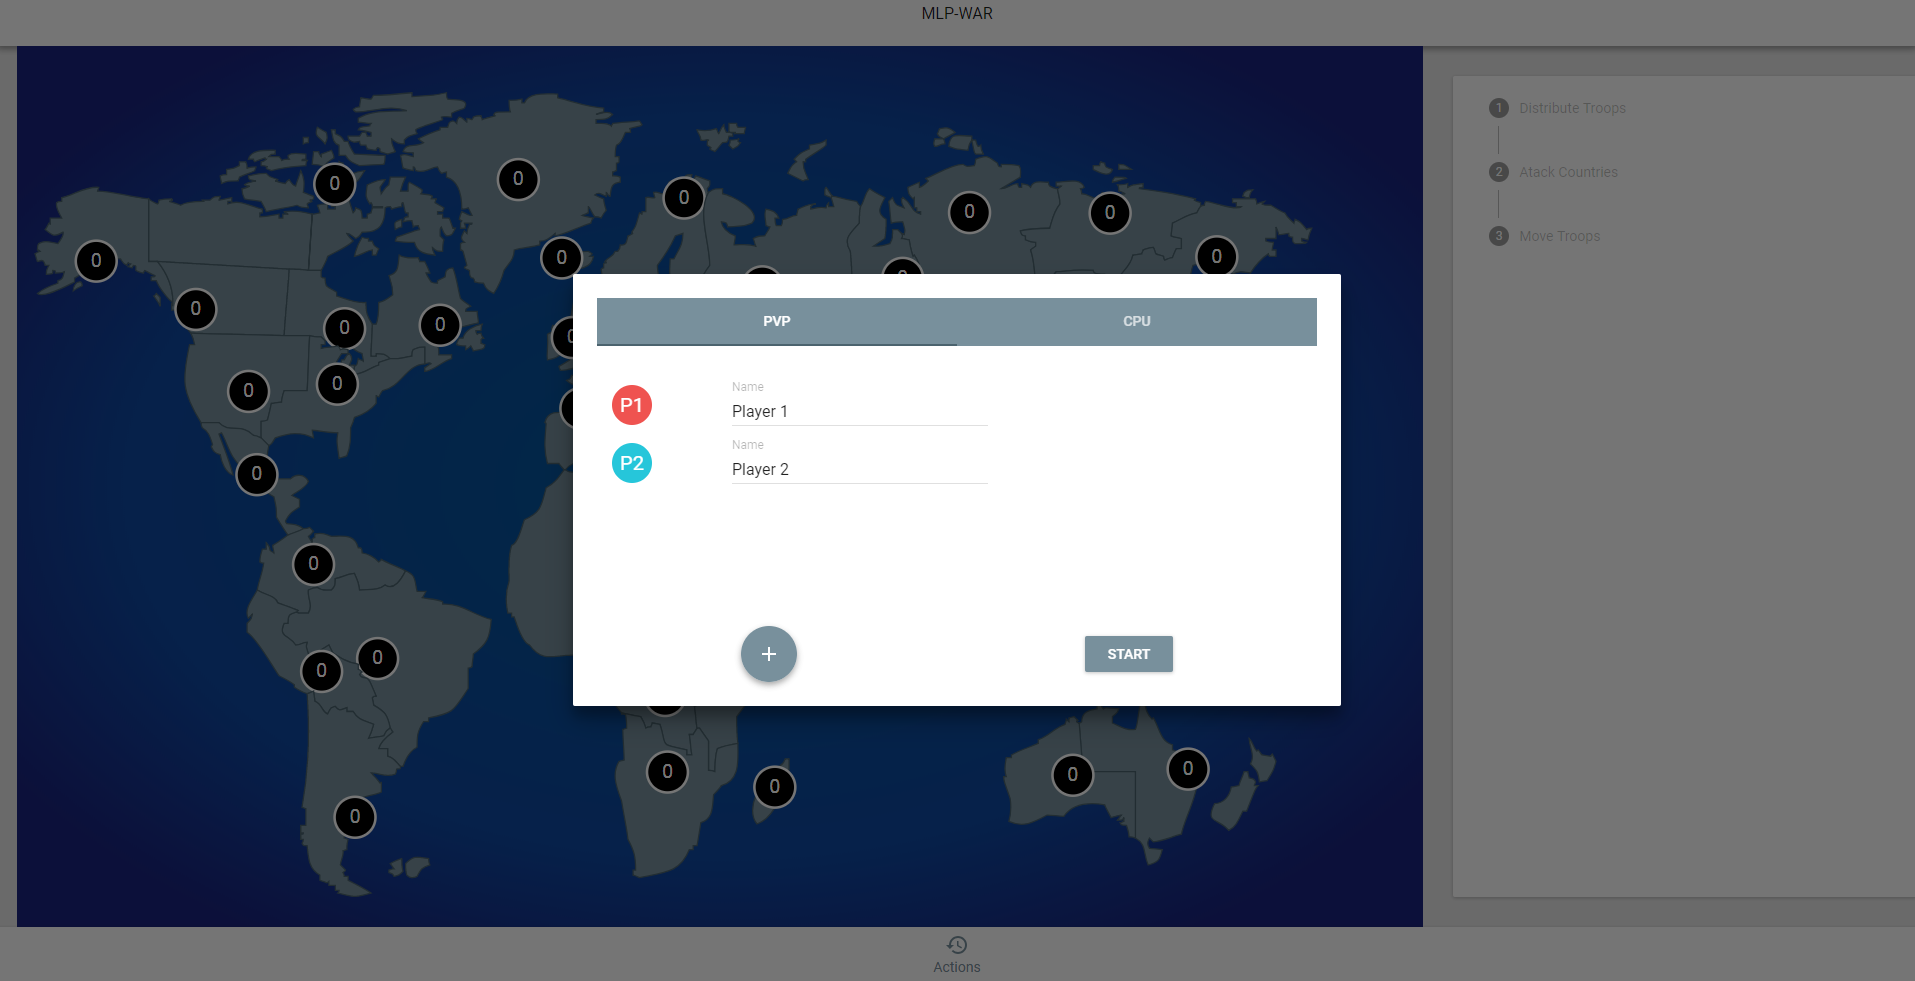
\includegraphics[width=1.0\textwidth]{images/landing.png}
  \caption{Página inicial}
  \label{fig:landing}
\end{figure}

Nessa etapa é possível adicionar novos jogadores e também renomeá-los. Caso se deseje adicionar jogadores controlados pela aplicação é necessário usar a aba CPU, onde é habilitada a alteração de modo de jogo de cada jogador.
A figura \ref{fig:setup} está uma configuração de exemplo.

\begin{figure}[h!]
\centering
  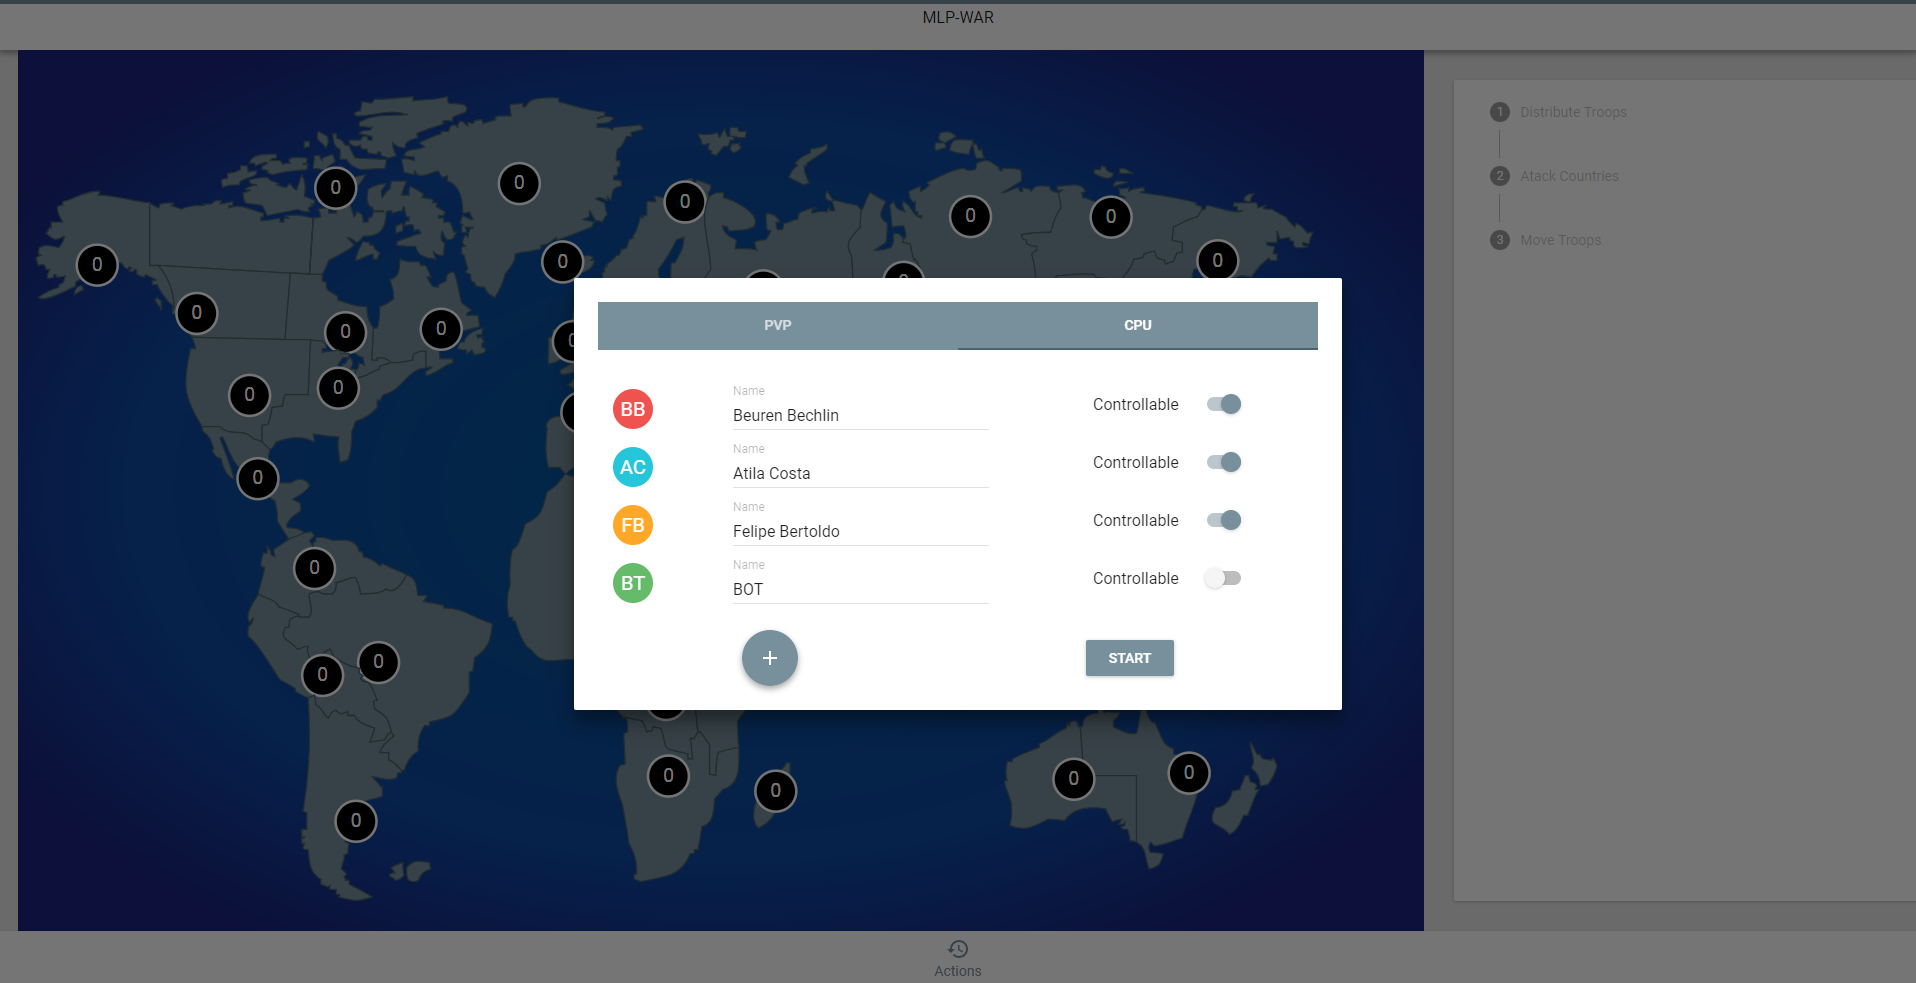
\includegraphics[width=1.0\textwidth]{images/setup.png}
  \caption{Configuração do jogo}
  \label{fig:setup}
\end{figure}

Ao iniciar o jogo cada jogador terá 1 minuto para realizar os passos de distribuição de tropas, ataque a inimigos e movimentação. Caso o tempo se esgote, a fase será automaticamente trocada para a próxima no fluxo normal de jogo entretanto, caso se deseje acelerar o processo, é possível usar o botão \textit{finish} para forçar a troca de etapa.
A ordem de jogadores é definida exatamente como a descrita na etapa de configuração do jogo.

Na figura \ref{fig:initGame} está retratado o início do jogo.

\begin{figure}[h!]
\centering
  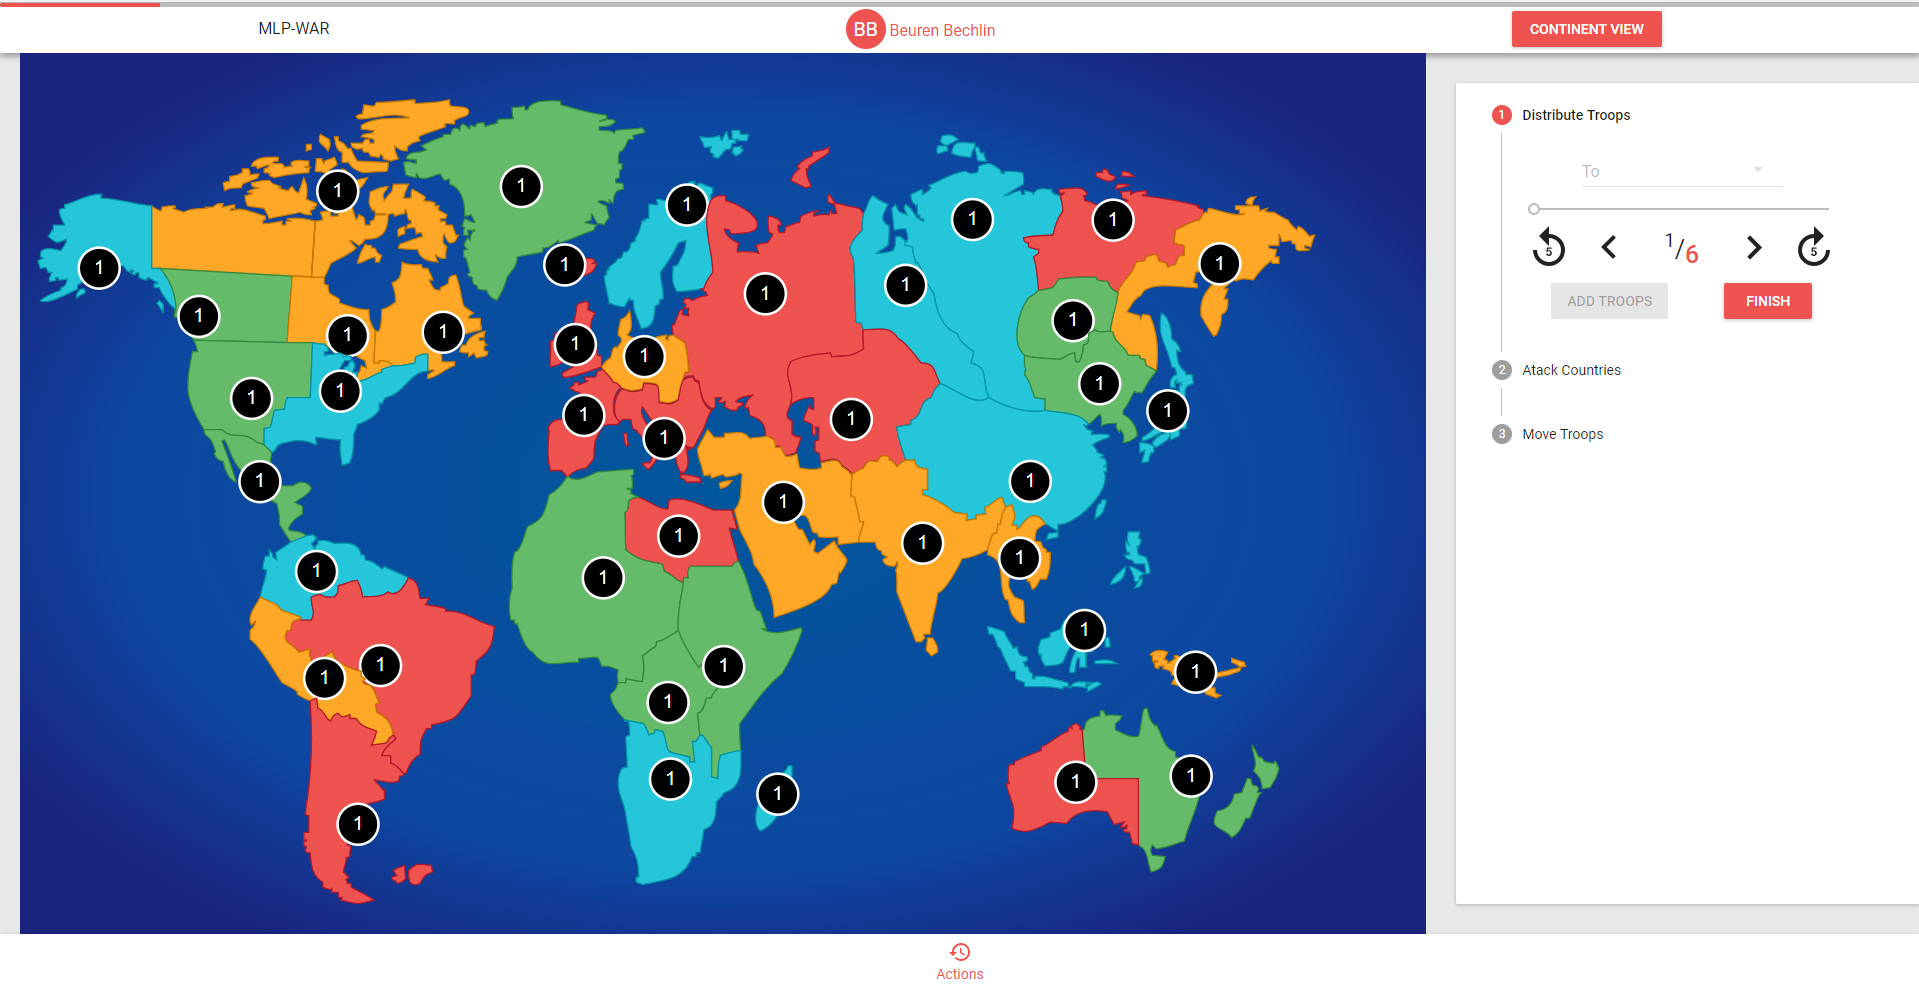
\includegraphics[width=1.0\textwidth]{images/initGame.png}
  \caption{Início do jogo}
  \label{fig:initGame}
\end{figure}

Ao lado direito da tela está o menu de ações do jogo, onde cada jogador pode realizar sua interação com o jogo. Outro meio de selecionar países é utilizando o mapa através do qual indicações visuais de quais países podem ser selecionados facilitam a visualização. Importante ressaltar é que caso se use as caixas de seleção os países também são ressaltados no mapa para facilitar a visualização.
Como a conquista de um continente inteiro influencia na quantidade de tropas recebidas o jogo disponibiliza uma forma de visualização por continentes para facilitar a visualização de fronteiras.
A figura \ref{fig:continentView} mostra a visualização em modo continente.

\begin{figure}[h!]
\centering
  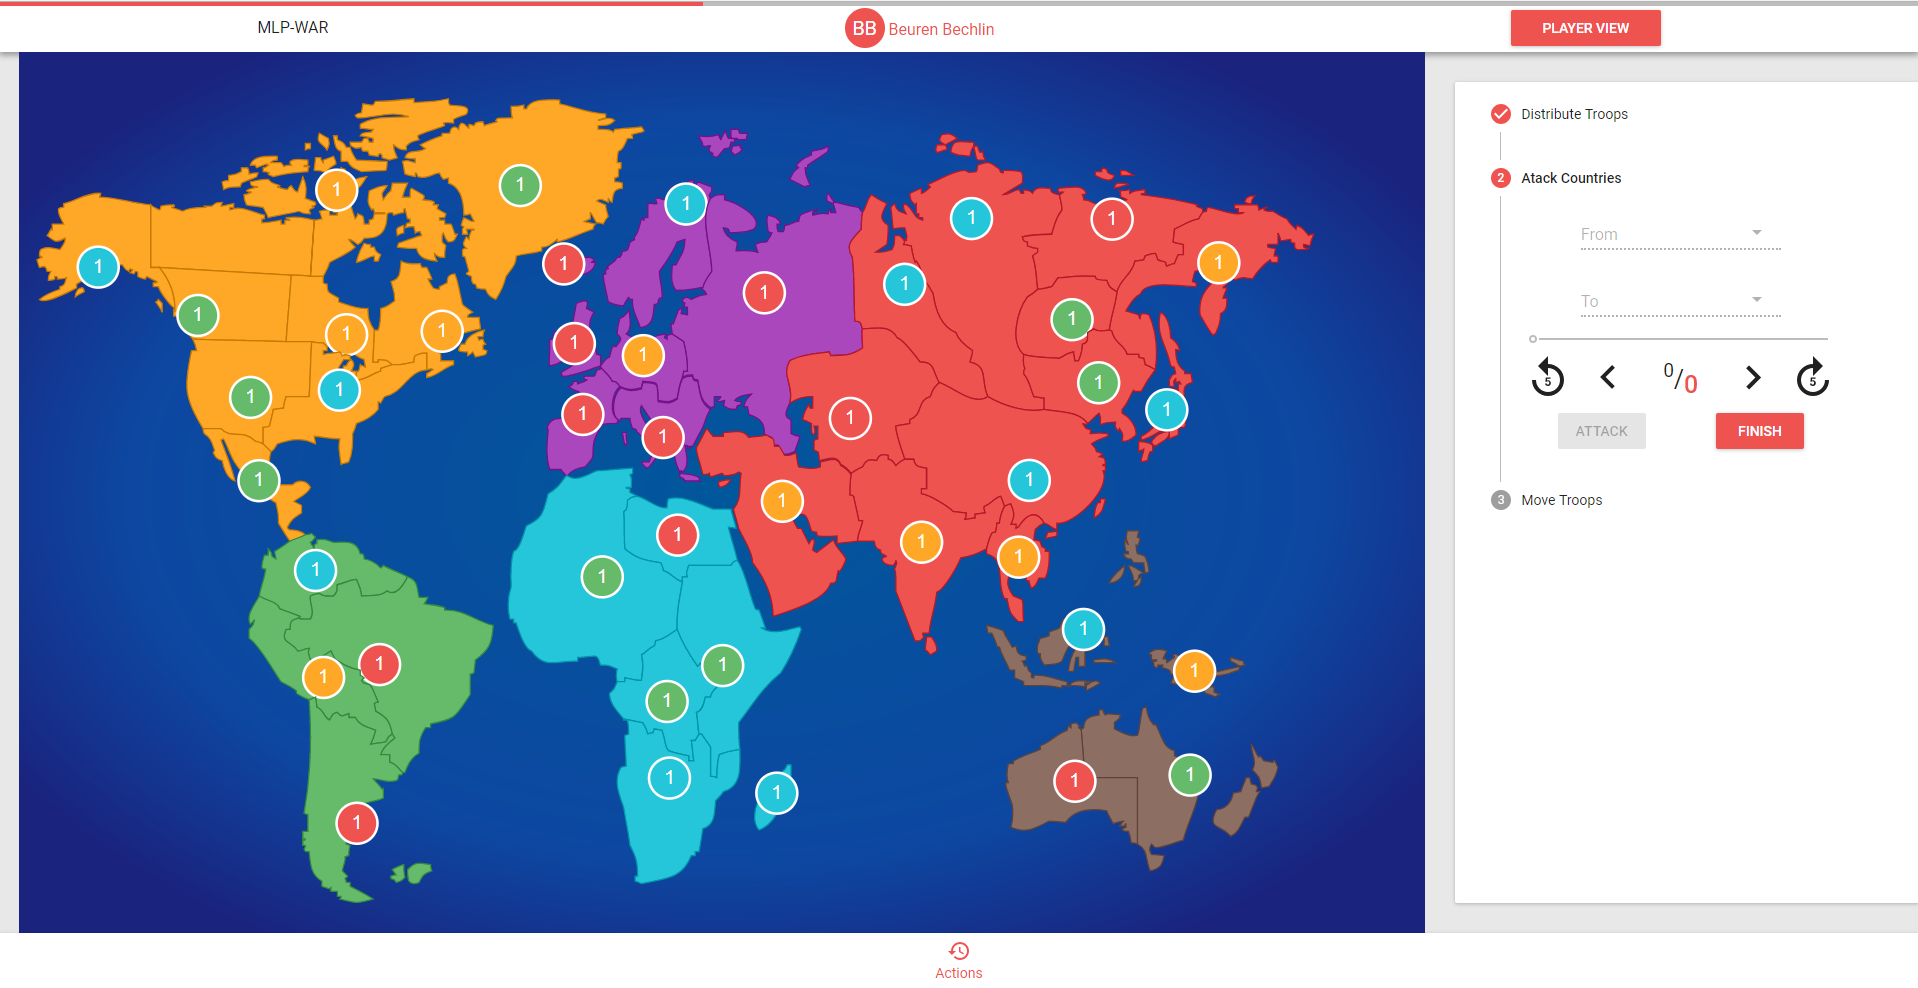
\includegraphics[width=1.0\textwidth]{images/continentView.png}
  \caption{Visualização em modo continente}
  \label{fig:continentView}
\end{figure}

A primeira etapa é a de distribuição de tropas, onde se seleciona um país que esteja sobre o controle do jogador ativo do turno, a quantidade de tropas que se deseja colocar nesse país e então se confirma a operação usando o botão "\textit{Add Troops}".
A figura \ref{fig:distribution} mostra esse etapa do jogo.

\begin{figure}[h!]
\centering
  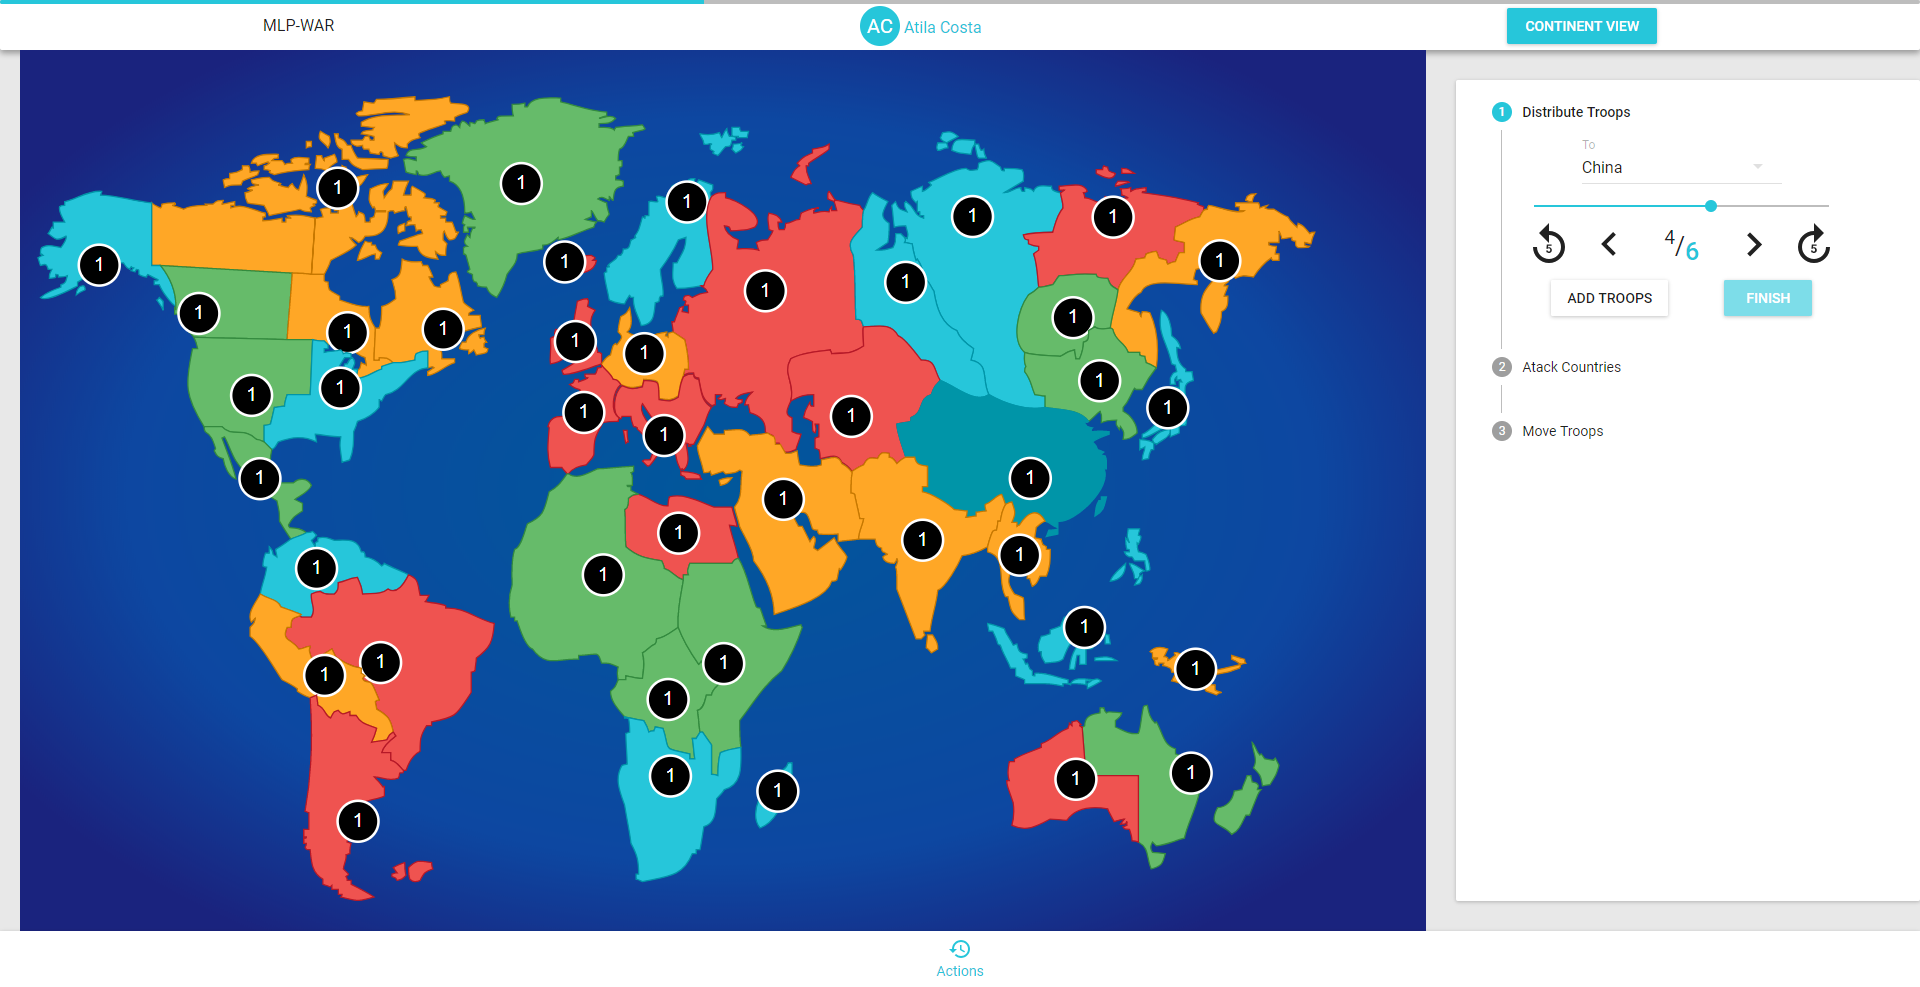
\includegraphics[width=1.0\textwidth]{images/distribution.png}
  \caption{Etapa de distribuição de tropas}
  \label{fig:distribution}
\end{figure}

A segunda etapa é o de ataque a países inimigos, onde se seleciona um país origem do jogador ativo no turno do jogo, um outro destino que não seja do jogador ativo, a quantidade de vezes que se deseja atacar e então se confirma a operação usando o botão "\textit{attack}". Importante ressaltar que ataques só podem ser realizados entre países que fazem fronteira. Para cada ataque é realizado um sorteio onde o defensor tem 55% de chances de vitória sobre o atacante, ou seja, caso se ataque 3 vezes um país para cada ataque será realizado o sorteio citado.A figura \ref{fig:attack} demonstra essa etapa.

\begin{figure}[h!]
\centering
  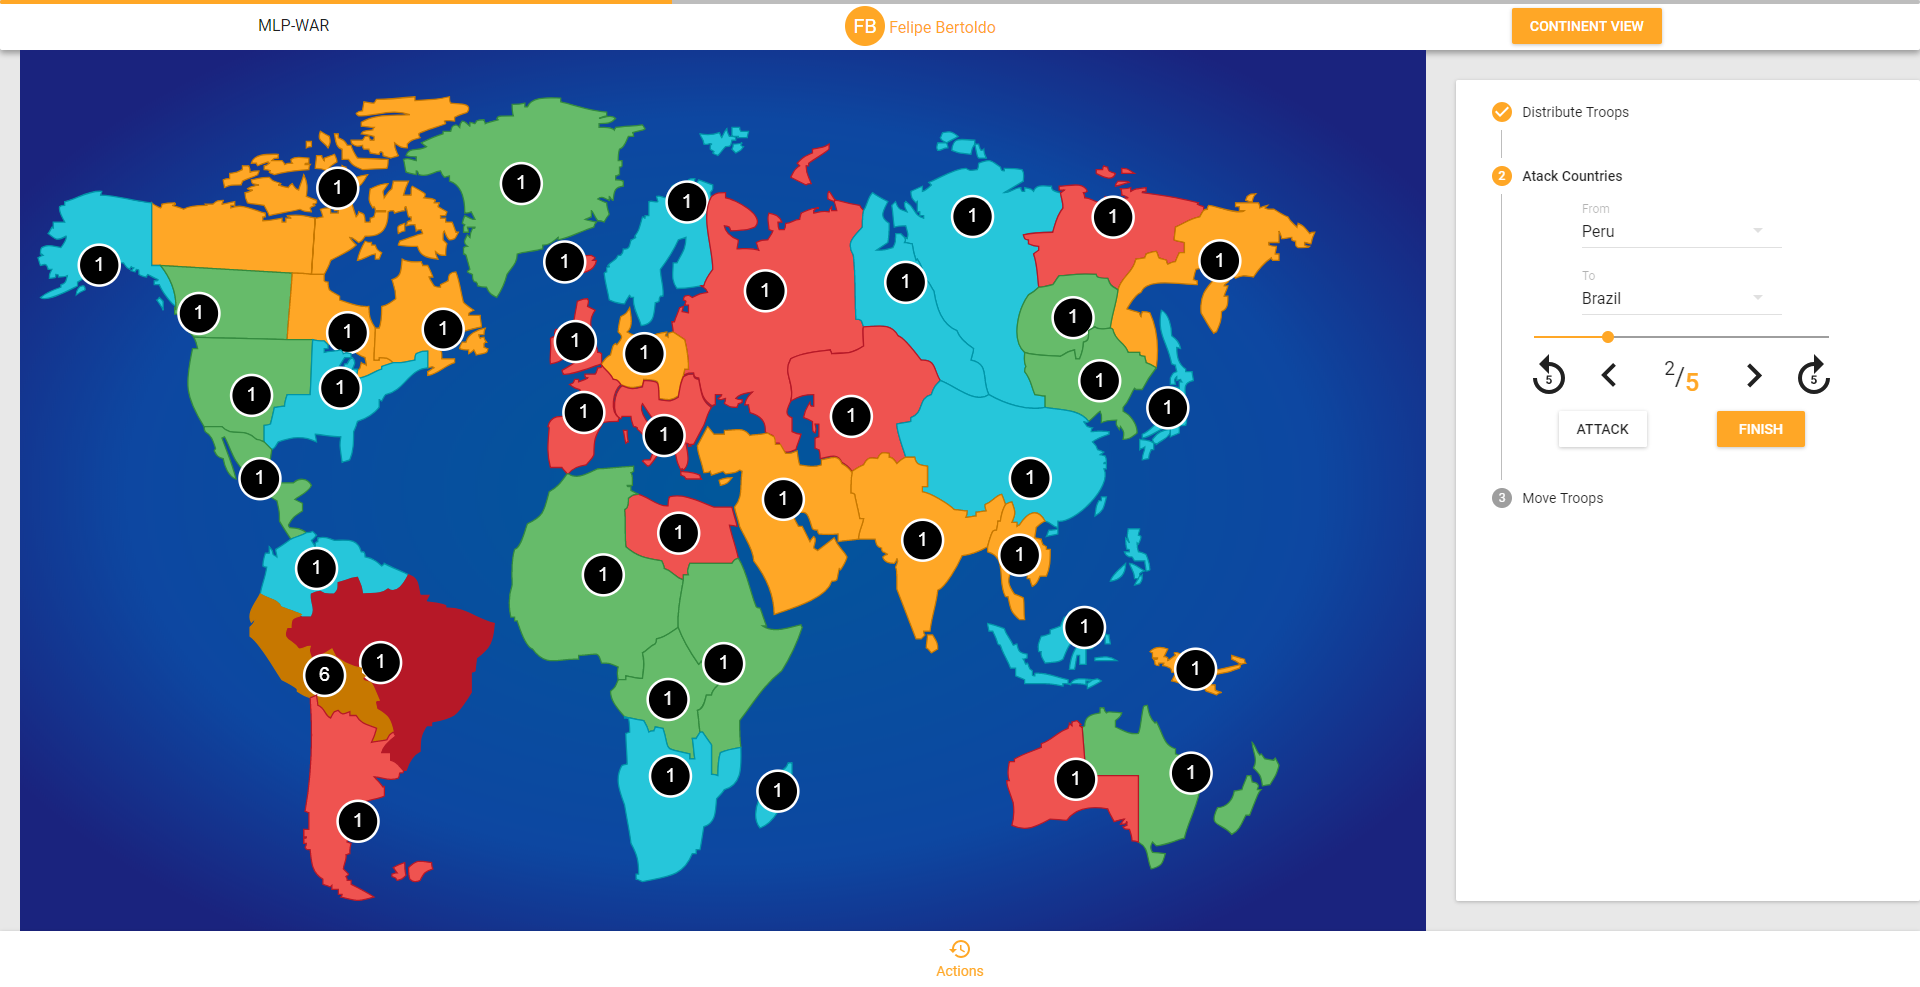
\includegraphics[width=1.0\textwidth]{images/attack.png}
  \caption{Etapa de ataque a países inimigos}
  \label{fig:attack}
\end{figure}

A última etapa é a de movimentação entre países aliados, onde se seleciona um país origem do jogador ativo no turno do jogo, um outro destino também do jogador ativo, a quantidade de tropas que se deseja mover e então se confirma a operação usando o botão "\textit{move}". As movimentações também só podem ser realizadas entre países que fazem fronteira.
A figura \ref{fig:move} retrata a fase de movimentação de tropas.

\begin{figure}[h!]
\centering
  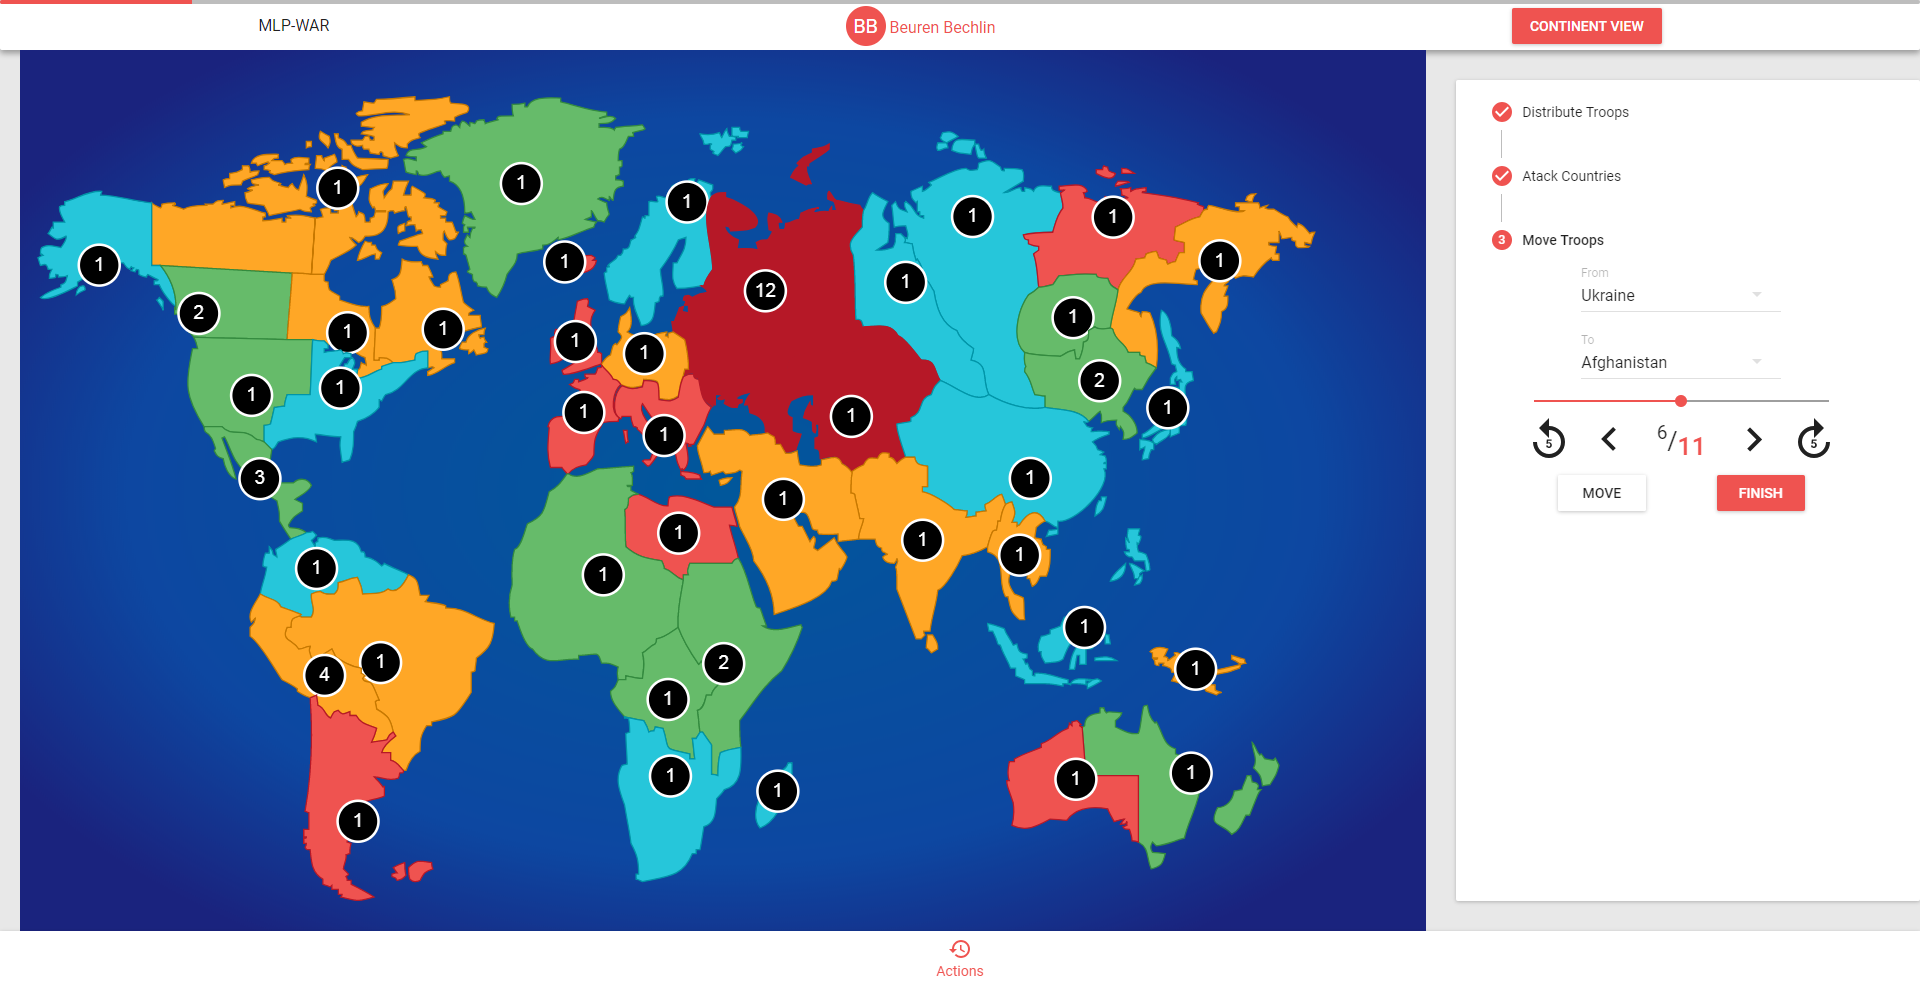
\includegraphics[width=1.0\textwidth]{images/move.png}
  \caption{Etapa de movimentação de tropas}
  \label{fig:move}
\end{figure}

Caso seja usado algum jogador controlado pelo computador, no turno desse jogador as ações serão bloqueadas pois são todas resolvidas pela própria aplicação.
A figura \label{fig:bot} mostra um jogador controlado pelo computador na etapa de ataque.

\begin{figure}[h!]
\centering
  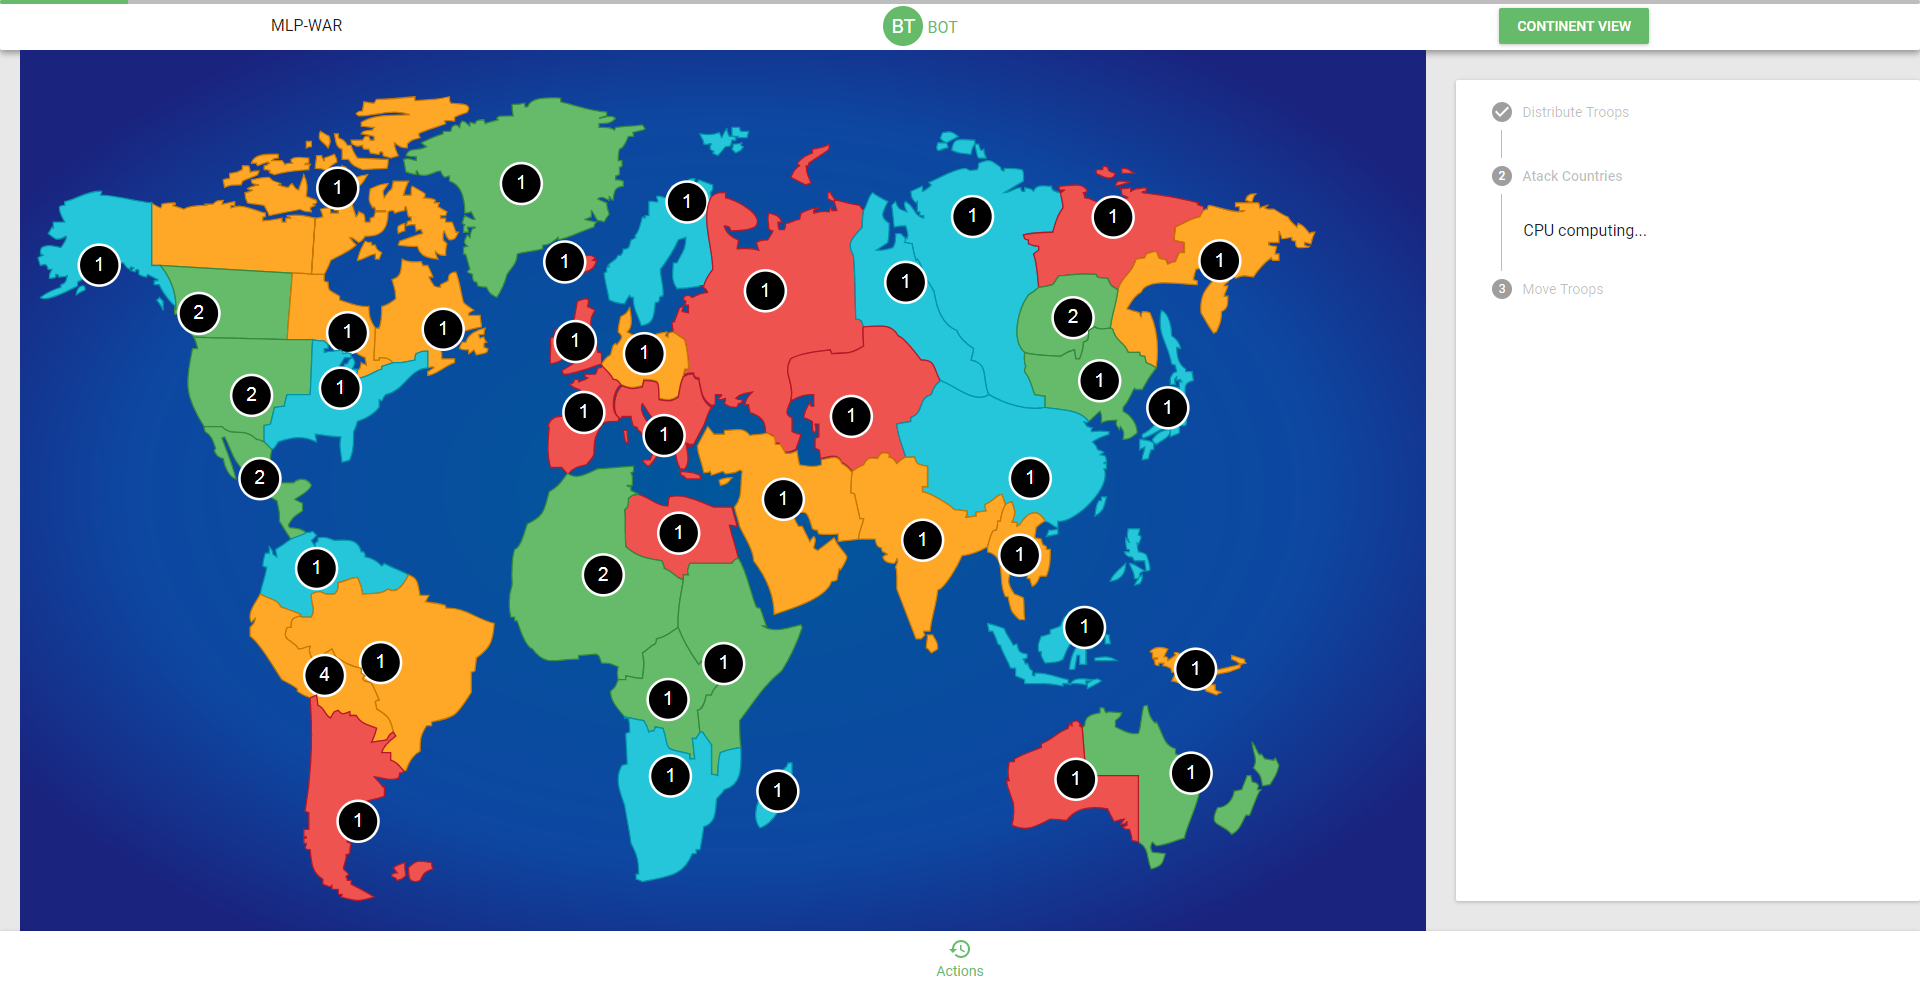
\includegraphics[width=1.0\textwidth]{images/bot.png}
  \caption{Turno do jogador controlado pelo computador}
  \label{fig:bot}
\end{figure}

O jogo termina quando um jogador conquistar todos os países e esse jogador é o vencedor.
A figura \label{fig:endGame} mostra o fim do jogo com o jogador chamado \textit{BOT} vencendo a partida.

\begin{figure}[h!]
\centering
  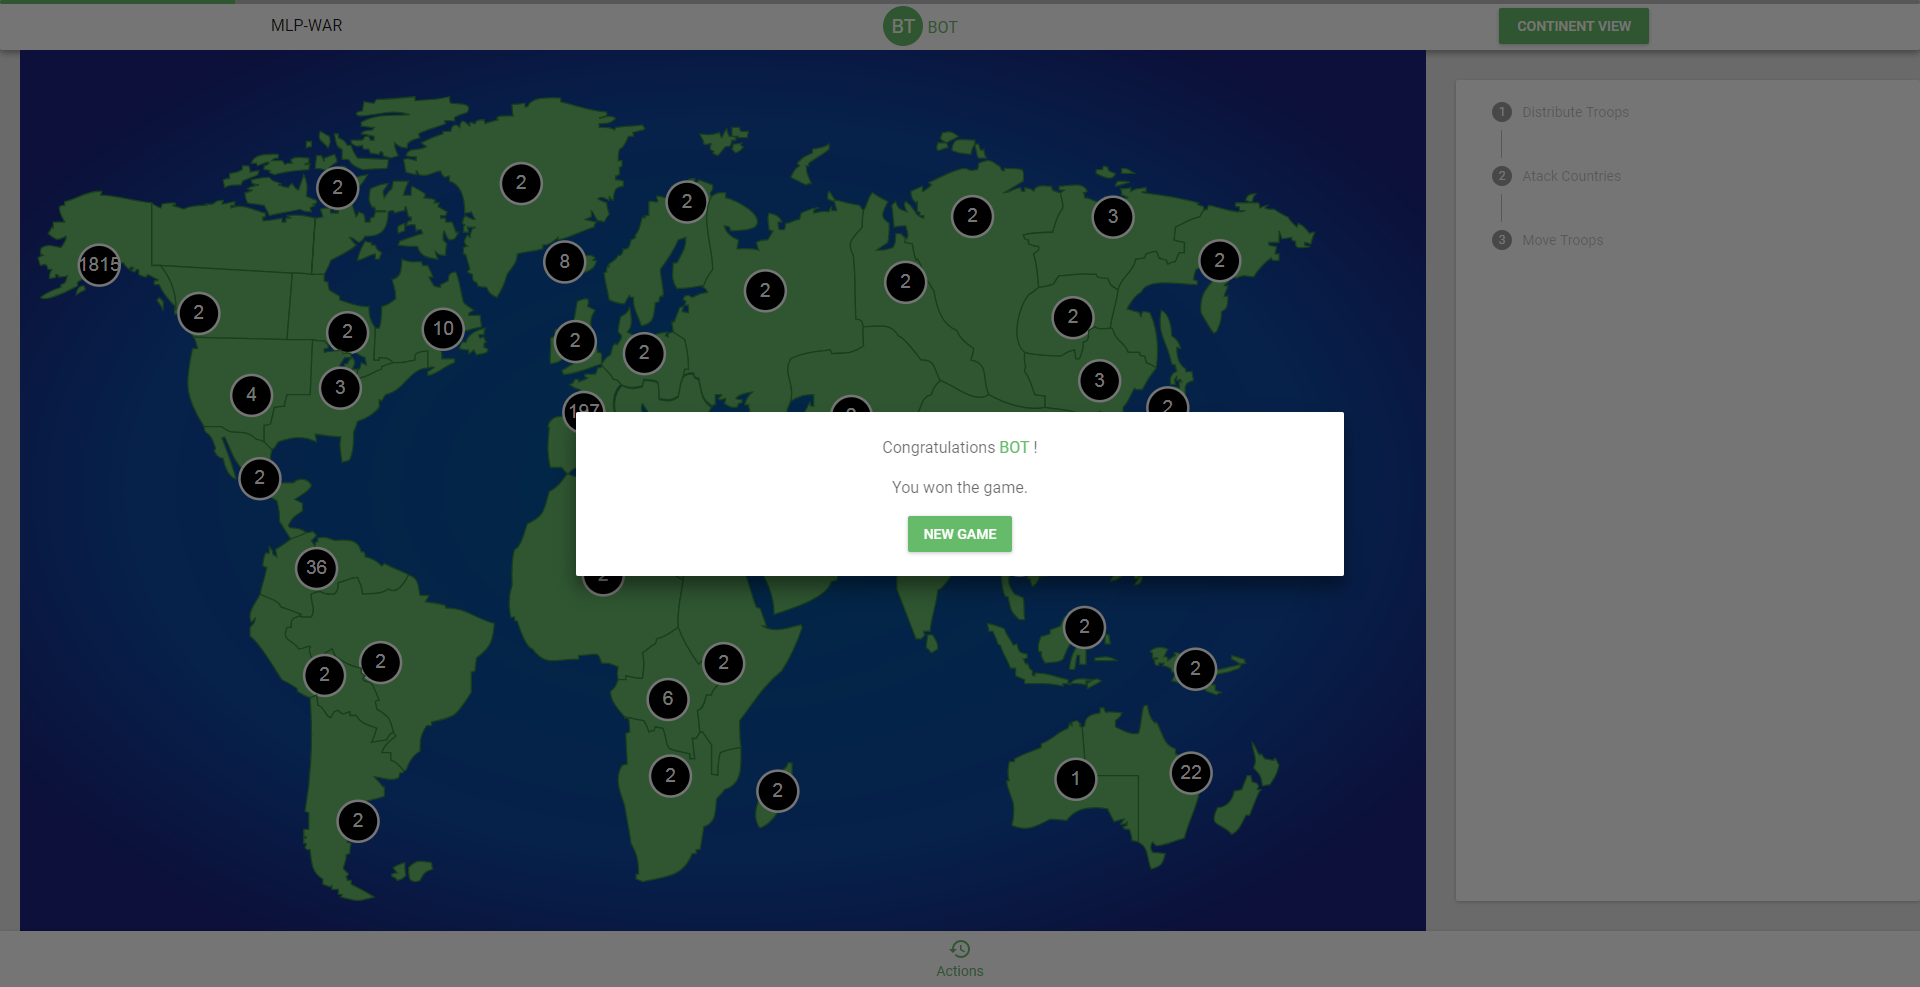
\includegraphics[width=1.0\textwidth]{images/endGame.png}
  \caption{Fim do jogo}
  \label{fig:endGame}
\end{figure}

\chapter{Conclusão}
Ao final do trabalho notamos que a linguagem é bem indicada para esse tipo de problema, com muita interação com o usuário e necessidade de lidar com ações disparadas assincronamente.
Ela possui um conceito interessante de pilha de execução, eventos e de animação que fazem com seja possível executar procedimentos com contextos totalmente diferentes mesmo que executando efetivamente sobre uma única thread.
Além disso possui um escalonador otimizado para interação com usuário possibilitando até mesmo uma fila específica para procedimentos de animação que tendem a ser escalonada a cada 1 / 60 segundos.
Isso também nos guiou para não criar grandes pontos de computação extensiva, já que no momento em que o procedimento entra em execução ele seguirá até encontrar um ponto de parada.
Mesmo tomando cuidado com essa limitação, esse problema pode ser notado quando um jogador é controlado pelo computador e realiza muitas ações em um curto espaço do tempo, fazendo assim que tanto a interação quanto a atualização da tela são congeladas rapidamente, esse problema é agravado com o aumento de países sobre o controle do computador. Isso poderia ser solucionado gerando eventos e dando um espaço de tempo entre as modificações, especificamente com o uso do comando timeout.
Nesse trabalho também podemos notar como a definição de uso de alguns \textit{frameworks} e bibliotecas podem acabar por guiar toda a solução.
Nesse contexto, o \verb|React| possui uma limitação quanto a entradas de valores em seus componentes, já que realiza otimizações para checar se houve diferenças nas entradas que devem disparar um novo ciclo de renderização do componente.
Dessa maneira, o \verb|React| sempre faz com que as variáveis de estados sejam de alguma forma observadas por ele e estejam disponíveis em toda a árvore de componentes. Isso acarreta a situação na qual caso alguma variável de estado seja alterada sem a devida notificação por algum agente externo não seja disparado nenhum novo ciclo de renderização.
Esse tipo de solução leva a uso extensivo de padrão de projeto \textit{singleton}, onde todos os componentes quando queiram usar algumas variáveis de estados acessem sempre a mesma instância que contenha essas variáveis.
Em relação ao Typescript concordamos que ele é importante para grandes projetos com times distribuídos em relação ao Javascript comum, adicionando  uma nova camada de verificação e garantia para os desenvolvedores com o uso de checagem estática. Entretanto, os conceitos introduzidos com a especificação ainda são bem novos, além da própria especificação estar evoluindo muito rapidamente. Por exemplo no início do projeto optamos por typescript 2.8.1 lançado em março de 2018 e nesse mês de junho de 2018 já se encontra na versão 2.9.2. Esse evolução rápida acaba gerando confusão, já que muitas das soluções proposta pela comunidade para integração com as bibliotecas e para a arquitetura de projeto sejam invalidadas ou devam sofrer atualização muito rapidamente. Isso gera um nível de insegurança ao desenvolver, já que é necessário ler muitos conteúdos diferentes para optar por um tipo de solução, e eles não possuem um feedback tão grande da comunidade sobre a dúvida de se essa escolha é realmente a melhor a ser tomada.

\bibliographystyle{abntex2-alf}

\begin{thebibliography}{9}
\bibitem{TypeScriptReference}
The TypeScript Reference,
\\\texttt{https://www.typescriptlang.org/docs/home.html}

\bibitem{ReactJSReference}
The ReactJS Reference,
\\\texttt{https://reactjs.org/docs/react-api.html}


\bibitem{ReduxWithReact}
Using Redux with React,
\\\texttt{https://redux.js.org/basics/usage-with-react}

\bibitem{UnderscoreJS}
Underscore JS,
\\\texttt{http://underscorejs.org/}

\bibitem{ReactReduxGuide}
React and Redux TypeScript Guide,
\\\texttt{https://github.com/piotrwitek/react-redux-typescript-guide}

\bibitem{patternmatching}
Pattern Matching with Typescript,
\\\texttt{https://pattern-matching-with-typescript.alabor.me/}



\end{thebibliography}


\end{document}
